% A LaTeX template for MSc Thesis submissions to 
% Politecnico di Milano (PoliMi) - School of Industrial and Information Engineering
%
% S. Bonetti, A. Gruttadauria, G. Mescolini, A. Zingaro
% e-mail: template-tesi-ingind@polimi.it
%
% Last Revision: October 2021
%
% Copyright 2021 Politecnico di Milano, Italy. NC-BY

\documentclass{Configuration_Files/PoliMi3i_thesis}

%------------------------------------------------------------------------------
%	REQUIRED PACKAGES AND  CONFIGURATIONS
%------------------------------------------------------------------------------

% CONFIGURATIONS
\usepackage[colorlinks=true, urlcolor=blue, linkcolor=red]{hyperref}
\usepackage{parskip} % For paragraph layout
\usepackage{setspace} % For using single or double spacing
\usepackage{emptypage} % To insert empty pages
\usepackage{graphicx}
\usepackage{subcaption}
\usepackage{multicol} % To write in multiple columns (executive summary)
\setlength\columnsep{15pt} % Column separation in executive summary
\setlength\parindent{0pt} % Indentation
\raggedbottom  

% PACKAGES FOR TITLES
\usepackage{titlesec}
% \titlespacing{\section}{left spacing}{before spacing}{after spacing}
\titlespacing{\section}{0pt}{3.3ex}{2ex}
\titlespacing{\subsection}{0pt}{3.3ex}{1.65ex}
\titlespacing{\subsubsection}{0pt}{3.3ex}{1ex}
\usepackage{color}

% PACKAGES FOR LANGUAGE AND FONT
\usepackage[english]{babel} % The document is in English  
\usepackage[utf8]{inputenc} % UTF8 encoding
\usepackage[T1]{fontenc} % Font encoding
\usepackage[11pt]{moresize} % Big fonts

% PACKAGES FOR IMAGES
\usepackage{graphicx}
\usepackage{listings}
\usepackage{xcolor}
\lstdefinestyle{json}{
    basicstyle=\ttfamily\scriptsize,
    stringstyle=\color{blue},
    numberstyle=\color{gray},
    stepnumber=1,
    numbersep=10pt,
    showstringspaces=false,
    breaklines=true,
    frame=lines,
    backgroundcolor=\color{background},
    literate=
     *{0}{{{\color{numb}0}}}{1}
      {1}{{{\color{numb}1}}}{1}
      {2}{{{\color{numb}2}}}{1}
      {3}{{{\color{numb}3}}}{1}
      {4}{{{\color{numb}4}}}{1}
      {5}{{{\color{numb}5}}}{1}
      {6}{{{\color{numb}6}}}{1}
      {7}{{{\color{numb}7}}}{1}
      {8}{{{\color{numb}8}}}{1}
      {9}{{{\color{numb}9}}}{1}
      {:}{{{\color{punct}{:}}}}{1}
      {,}{{{\color{punct}{,}}}}{1}
      {\{}{{{\color{delim}{\{}}}}{1}
      {\}}{{{\color{delim}{\}}}}}{1}
      {[}{{{\color{delim}{[}}}}{1}
      {]}{{{\color{delim}{]}}}}{1},
}

% Define colors
\definecolor{background}{HTML}{EEEEEE}
\definecolor{delim}{RGB}{20,105,176}
\colorlet{numb}{magenta}
\colorlet{punct}{red}
\colorlet{str}{blue}

\documentclass{article}
\usepackage{listings}
\usepackage{xcolor}
\usepackage{upquote} % Use this to handle straight quotes in verbatim environments

% Define colors
\definecolor{commentcolor}{RGB}{0,128,0}
\definecolor{stringcolor}{RGB}{255,0,0}
\definecolor{keywordcolor}{RGB}{0,0,255}
\definecolor{backgroundcolor}{RGB}{245,245,245}

% Define Cypher language style
\lstdefinelanguage{Cypher}{
    keywords={MATCH, CREATE, DETACH, DELETE, WHERE, AND, OR, NOT, RETURN, DISTINCT, AS, ORDER, BY, SET, WITH, LIMIT, SKIP, IN, UNWIND, MERGE, ON, CASE, WHEN, THEN, ELSE, END, DESC, ASC},
    keywordstyle=\color{keywordcolor}\bfseries,
    ndkeywords={node, relationship},
    ndkeywordstyle=\color{cyan}\bfseries,
    identifierstyle=\color{black},
    sensitive=false,
    comment=[l]{//},
    commentstyle=\color{commentcolor}\ttfamily,
    stringstyle=\color{stringcolor}\ttfamily,
    morestring=[b]',
    morestring=[b]"
}

% Code listing style
\lstset{
    language=Cypher,
    extendedchars=true,
    basicstyle=\ttfamily\scriptsize,
    showstringspaces=false,
    showspaces=false,
    numbers=left,
    numberstyle=\footnotesize,
    numbersep=9pt,
    tabsize=2,
    breaklines=true,
    showtabs=false,
    captionpos=b,
    backgroundcolor=\color{backgroundcolor}
}



\usepackage{transparent} % Enables transparent images
\usepackage{eso-pic} % For the background picture on the title page
\usepackage{subfig} % Numbered and caption subfigures using \subfloat.
\usepackage{tikz} % A package for high-quality hand-made figures.
\usetikzlibrary{}
\graphicspath{{./Images/}} % Directory of the images
\usepackage{caption} % Coloured captions
\usepackage{xcolor} % Coloured captions
\usepackage{amsthm,thmtools,xcolor} % Coloured "Theorem"
\usepackage{float}

% STANDARD MATH PACKAGES
\usepackage{amsmath}
\usepackage{amsthm}
\usepackage{amssymb}
\usepackage{amsfonts}
\usepackage{bm}
\usepackage[overload]{empheq} % For braced-style systems of equations.
\usepackage{fix-cm} % To override original LaTeX restrictions on sizes

% PACKAGES FOR TABLES
\usepackage{tabularx}
\usepackage{longtable} % Tables that can span several pages
\usepackage{colortbl}

% PACKAGES FOR ALGORITHMS (PSEUDO-CODE)
\usepackage{algorithm}
\usepackage{algorithmic}

% PACKAGES FOR REFERENCES & BIBLIOGRAPHY
\usepackage[colorlinks=true,linkcolor=black,anchorcolor=black,citecolor=black,filecolor=black,menucolor=black,runcolor=black,urlcolor=black]{hyperref} % Adds clickable links at references
\usepackage{cleveref}
\usepackage[square, numbers, sort&compress]{natbib} % Square brackets, citing references with numbers, citations sorted by appearance in the text and compressed
\bibliographystyle{abbrvnat} % You may use a different style adapted to your field

% OTHER PACKAGES
\usepackage{pdfpages} % To include a pdf file
\usepackage{afterpage}
\usepackage{lipsum} % DUMMY PACKAGE
\usepackage{fancyhdr} % For the headers
\fancyhf{}

% Input of configuration file. Do not change config.tex file unless you really know what you are doing. 
% Define blue color typical of polimi
\definecolor{bluepoli}{cmyk}{0.4,0.1,0,0.4}

% Custom theorem environments
\declaretheoremstyle[
  headfont=\color{bluepoli}\normalfont\bfseries,
  bodyfont=\color{black}\normalfont\itshape,
]{colored}

% Set-up caption colors
\captionsetup[figure]{labelfont={color=bluepoli}} % Set colour of the captions
\captionsetup[table]{labelfont={color=bluepoli}} % Set colour of the captions
\captionsetup[algorithm]{labelfont={color=bluepoli}} % Set colour of the captions

\theoremstyle{colored}
\newtheorem{theorem}{Theorem}[chapter]
\newtheorem{proposition}{Proposition}[chapter]

% Enhances the features of the standard "table" and "tabular" environments.
\newcommand\T{\rule{0pt}{2.6ex}}
\newcommand\B{\rule[-1.2ex]{0pt}{0pt}}

% Pseudo-code algorithm descriptions.
\newcounter{algsubstate}
\renewcommand{\thealgsubstate}{\alph{algsubstate}}
\newenvironment{algsubstates}
  {\setcounter{algsubstate}{0}%
   \renewcommand{\STATE}{%
     \stepcounter{algsubstate}%
     \Statex {\small\thealgsubstate:}\space}}
  {}

% New font size
\newcommand\numfontsize{\@setfontsize\Huge{200}{60}}

% Title format: chapter
\titleformat{\chapter}[hang]{
\fontsize{50}{20}\selectfont\bfseries\filright}{\textcolor{bluepoli} \thechapter\hsp\hspace{2mm}\textcolor{bluepoli}{|   }\hsp}{0pt}{\huge\bfseries \textcolor{bluepoli}
}

% Title format: section
\titleformat{\section}
{\color{bluepoli}\normalfont\Large\bfseries}
{\color{bluepoli}\thesection.}{1em}{}

% Title format: subsection
\titleformat{\subsection}
{\color{bluepoli}\normalfont\large\bfseries}
{\color{bluepoli}\thesubsection.}{1em}{}

% Title format: subsubsection
\titleformat{\subsubsection}
{\color{bluepoli}\normalfont\large\bfseries}
{\color{bluepoli}\thesubsubsection.}{1em}{}

% Shortening for setting no horizontal-spacing
\newcommand{\hsp}{\hspace{0pt}}

\makeatletter
% Renewcommand: cleardoublepage including the background pic
\renewcommand*\cleardoublepage{%
  \clearpage\if@twoside\ifodd\c@page\else
  \null
  \AddToShipoutPicture*{\BackgroundPic}
  \thispagestyle{empty}%
  \newpage
  \if@twocolumn\hbox{}\newpage\fi\fi\fi}
\makeatother

%For correctly numbering algorithms
\numberwithin{algorithm}{chapter}

%----------------------------------------------------------------------------
%	NEW COMMANDS DEFINED
%----------------------------------------------------------------------------

% EXAMPLES OF NEW COMMANDS
\newcommand{\bea}{\begin{eqnarray}} % Shortcut for equation arrays
\newcommand{\eea}{\end{eqnarray}}
\newcommand{\e}[1]{\times 10^{#1}}  % Powers of 10 notation

%----------------------------------------------------------------------------
%	ADD YOUR PACKAGES (be careful of package interaction)
%----------------------------------------------------------------------------

%----------------------------------------------------------------------------
%	ADD YOUR DEFINITIONS AND COMMANDS (be careful of existing commands)
%----------------------------------------------------------------------------

%----------------------------------------------------------------------------
%	BEGIN OF YOUR DOCUMENT
%----------------------------------------------------------------------------

\begin{document}

\fancypagestyle{plain}{%
\fancyhf{} % Clear all header and footer fields
\fancyhead[RO,RE]{\thepage} %RO=right odd, RE=right even
\renewcommand{\headrulewidth}{0pt}
\renewcommand{\footrulewidth}{0pt}}

%----------------------------------------------------------------------------
%	TITLE PAGE
%----------------------------------------------------------------------------

\pagestyle{empty} % No page numbers
\frontmatter % Use roman page numbering style (i, ii, iii, iv...) for the preamble pages

\puttitle{
	title=Systems and Methods for Big and Unstructured Data Project,
	name1=Mehmet Emre Akbulut \small(10972566), % Author Name and Surname
	name2=Yavuz Samet Topcuoglu \small(10967930),
	academicyear=2023-2024,
} % These info will be put into your Title page 

%----------------------------------------------------------------------------
%	PREAMBLE PAGES: ABSTRACT (inglese e italiano), EXECUTIVE SUMMARY
%----------------------------------------------------------------------------
\startpreamble
\setcounter{page}{1} % Set page counter to 1

%----------------------------------------------------------------------------
%	LIST OF CONTENTS/FIGURES/TABLES/SYMBOLS
%----------------------------------------------------------------------------

% TABLE OF CONTENTS
\thispagestyle{empty}
\tableofcontents % Table of contents 
\thispagestyle{empty}
\cleardoublepage

%-------------------------------------------------------------------------
%	THESIS MAIN TEXT
%-------------------------------------------------------------------------
% In the main text of your thesis you can write the chapters in two different ways:
%
%(1) As presented in this template you can write:
%    \chapter{Title of the chapter}
%    *body of the chapter*
%
%(2) You can write your chapter in a separated .tex file and then include it in the main file with the following command:
%    \chapter{Title of the chapter}
%    \input{chapter_file.tex}
%
% Especially for long thesis, we recommend you the second option.

\addtocontents{toc}{\vspace{2em}} % Add a gap in the Contents, for aesthetics
\mainmatter % Begin numeric (1,2,3...) page numbering


\chapter{Introduction}

Upon the delivery of the project, choosing a dataset in the field of football was a no-brainer for us, considering our enthusiasm for the game of football. The main aspect to take into consideration during the selection of the dataset was that it should be suitable for football analytics and that we should be able to find answers to the questions in our minds.

Graph databases excel in managing and interpreting complex relationships and interconnected data. Unlike traditional relational databases, they allow for more flexible and efficient handling of data that is naturally interconnected. That is exactly why we chose to use a graph database because of the nature of our dataset, which includes a multitude of interrelated elements and relationships.

Neo4j, a leading graph database technology, was selected for its robust performance, ease of query language, strong documentation, and existence of materials provided by the lecturers. Its ability to represent complex networks of data as graphs rather than tables makes it an ideal choice for our needs. Neo4j offers powerful querying capabilities through its Cypher language, making it possible to intuitively extract complex relationships and patterns from our dataset.

In conclusion, the choice of a graph database, and Neo4j in particular, aligns perfectly with our dataset's features and our project goals. The flexibility, efficiency, and intuitive nature of Neo4j enable us to delve deeper into the dataset, uncovering valuable insights that would be difficult to extract using other database technologies.




\chapter{Dataset}

You can find the dataset used in the project from \href{https://www.kaggle.com/datasets/davidcariboo/player-scores/data}{this link.}

The dataset has 9 CSV files, each file can be demonstrated with the following tables: \newline
\footnotesize{Note: The following figures contain only the column names of the respective csv files.}

\begin{figure}[H]
    \centering
    \includegraphics[width=1\linewidth]{Project Template/Images/appearances.png}
    \caption{Columns of appearances.csv}
\end{figure}

\begin{figure}[H]
    \centering
    
\includegraphics[width=1\linewidth]{Project Template/Images/club_games.png}
    \caption{Columns of club\_games.csv}
\end{figure}

\begin{figure}[H]
    \centering
    
\includegraphics[width=1\linewidth]{Project Template/Images/clubs1.png}
    
\includegraphics[width=1\linewidth]{Project Template/Images/clubs2.png}
\caption{Columns of clubs.csv}
\end{figure}

\begin{figure}[H]
    \centering
    
\includegraphics[width=1\linewidth]{Project Template/Images/competitions.png}
\caption{Columns of competitions.csv}
\end{figure}

\begin{figure}[H]
    \centering
    
\includegraphics[width=1\linewidth]{Project Template/Images/game_events.png}
\caption{Columns of game\_events.csv}
\end{figure}

\begin{figure}[H]
    \centering
    
\includegraphics[width=1\linewidth]{Project Template/Images/lineups.png}
\caption{Columns of game\_lineups.csv}
\end{figure}

\begin{figure}[H]
    \centering
    
\includegraphics[width=1\linewidth]{Project Template/Images/games1.png}
    
\includegraphics[width=1\linewidth]{Project Template/Images/games2.png}
    
\includegraphics[width=1\linewidth]{Project Template/Images/games3.png}
\caption{Columns of games.csv}
\end{figure}

\begin{figure}[H]
    \centering
    
\includegraphics[width=1\linewidth]{Project Template/Images/valuations.png}
\caption{Columns of player\_valuations.csv}
\end{figure}

\begin{figure}[H]
    \centering
    
\includegraphics[width=1\linewidth]{Project Template/Images/player1.png}
    
\includegraphics[width=1\linewidth]{Project Template/Images/player2.png}
    
\includegraphics[width=1\linewidth]{Project Template/Images/player3.png}
\caption{Columns of players.csv}
\end{figure}

Using these tables, we decided to create the following entities with respective attributes using Python scripts:


\begin{figure}[htbp]
  \centering
  % First row with 4 subfigures, each taking up 0.2 of the text width
  \begin{subfigure}[b]{0.2\linewidth}
    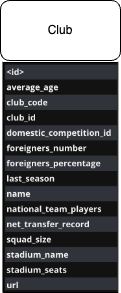
\includegraphics[width=\linewidth]{Project Template/Images/entities/club.drawio.png}
  \end{subfigure}
  \hfill
  \begin{subfigure}[b]{0.2\linewidth}
    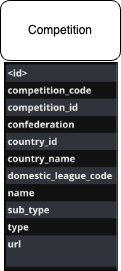
\includegraphics[width=\linewidth]{Project Template/Images/entities/comp.drawio.png}
  \end{subfigure}
  \hfill
  \begin{subfigure}[b]{0.23\linewidth}
    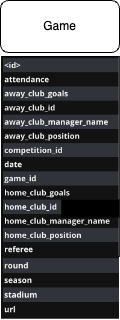
\includegraphics[width=\linewidth]{Project Template/Images/entities/game.drawio.png}
  \end{subfigure}
  \hfill
  \begin{subfigure}[b]{0.25\linewidth}
    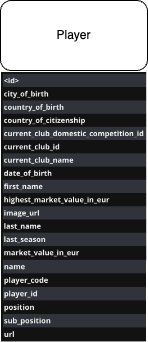
\includegraphics[width=\linewidth]{Project Template/Images/entities/player.drawio.png}
  \end{subfigure}
  
  % Add some space before the next row
  \vspace{1em}
  
  % Second row with 5 subfigures, each taking up 0.16 of the text width
  \begin{subfigure}[b]{0.12\linewidth}
    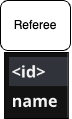
\includegraphics[width=\linewidth]{Project Template/Images/entities/ref.drawio.png}
  \end{subfigure}
  \hfill
  \begin{subfigure}[b]{0.24\linewidth}
    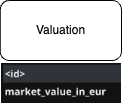
\includegraphics[width=\linewidth]{Project Template/Images/entities/val.drawio.png}
  \end{subfigure}
  \hfill
  \begin{subfigure}[b]{0.12\linewidth}
    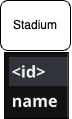
\includegraphics[width=\linewidth]{Project Template/Images/entities/stad.drawio.png}
  \end{subfigure}
  \hfill
  \begin{subfigure}[b]{0.2\linewidth}
    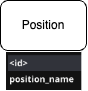
\includegraphics[width=\linewidth]{Project Template/Images/entities/position.drawio.png}
  \end{subfigure}
  \hfill
  \begin{subfigure}[b]{0.12\linewidth}
    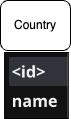
\includegraphics[width=\linewidth]{Project Template/Images/entities/country.drawio.png}
  \end{subfigure}
  
  \caption{Entities and their attributes.}
\end{figure}

\newpage

Please note that all entities and relationships have \textit{<id>} attribute. Since it is common to all different type of entities and relationships, it will not be included in the tables below. \textit{<id>} has type String.

\subsection*{Club}
\begin{longtable}{|p{4cm}|p{3cm}|p{8cm}|}
\hline
\textbf{Attribute} & \textbf{Type} & \textbf{Description} \\
\hline
\endhead
average\_age & Float & The average age of the club's players. \\
club\_code & String & The code representing the club. \\
club\_id & Integer & Unique identifier for the club. \\
domestic\_competition\_id & Integer & Identifier for the club's domestic competition. \\
foreigners\_number & Integer & Number of foreign players in the club. \\
foreigners\_percentage & Float & Percentage of foreign players in the club. \\
last\_season & Integer & The last season the club was active. \\
name & String & Full name of the club. \\
national\_team\_players & Integer & Number of players in the club who are also national team players. \\
net\_transfer\_record & Integer & Net amount spent on transfers (in EUR). \\
squad\_size & Integer & Total number of players in the club. \\
stadium\_name & String & Name of the club's stadium. \\
stadium\_seats & Integer & Number of seats in the club's stadium. \\
url & String & URL to the club's official website. \\
\hline
\end{longtable}

\subsection*{Competition}
\begin{longtable}{|p{4cm}|p{3cm}|p{8cm}|}
\hline
\textbf{Attribute} & \textbf{Type} & \textbf{Description} \\
\hline
\endhead
competition\_code & String & A unique code assigned to the competition. \\
competition\_id & Integer & The unique identifier for the competition. \\
confederation & String & The confederation to which the competition belongs. \\
country\_id & Integer & The identifier for the country where the competition is held. \\
country\_name & String & The name of the country where the competition is held. \\
domestic\_league\_code & String & A unique code representing the domestic league of the competition. \\
name & String & The official name of the competition. \\
sub\_type & String & Subcategory or type of the competition if any. \\
type & String & The type of competition, e.g., league, cup. \\
url & String & The URL to the competition's official webpage. \\
\hline
\end{longtable}

\newpage

\subsection*{Game}
\begin{longtable}{|p{5cm}|p{2cm}|p{8cm}|}
\hline
\textbf{Attribute} & \textbf{Type} & \textbf{Description} \\
\hline
\endhead
attendance & Integer & The number of people who attended the game. \\
away\_club\_goals & Integer & The number of goals scored by the away club. \\
away\_club\_id & Integer & Unique identifier for the away club. \\
away\_club\_manager\_name & String & The name of the manager of the away club. \\
away\_club\_position & String & The league position of the away club at the time of the game. \\
competition\_id & Integer & Identifier for the competition in which the game is played. \\
date & Date & The date on which the game was played. \\
game\_id & Integer & Unique identifier for the game. \\
home\_club\_goals & Integer & The number of goals scored by the home club. \\
home\_club\_id & Integer & Unique identifier for the home club. \\
home\_club\_manager\_name & String & The name of the manager of the home club. \\
home\_club\_position & String & The league position of the home club at the time of the game. \\
referee & String & The name of the referee for the game. \\
round & String & The round of the competition in which the game took place. \\
season & String & The season during which the game was played. \\
stadium & String & The stadium where the game was played. \\
url & String & The URL to the webpage with details about the game. \\
\hline
\end{longtable}


\subsection*{Position}
\begin{longtable}{|p{4cm}|p{3cm}|p{8cm}|}
\hline
\textbf{Attribute} & \textbf{Type} & \textbf{Description} \\
\hline
\endhead
position\_name & String & The name of the position. \\
\hline
\end{longtable}

\subsection*{Country}
\begin{longtable}{|p{4cm}|p{3cm}|p{8cm}|}
\hline
\textbf{Attribute} & \textbf{Type} & \textbf{Description} \\
\hline
\endhead
name & String & The name of the country. \\
\hline
\end{longtable}

\newpage

\subsection*{Player}
\begin{longtable}{|p{6.2cm}|p{1.6cm}|p{8cm}|}
\hline
\textbf{Attribute} & \textbf{Type} & \textbf{Description} \\
\hline
\endhead
city\_of\_birth & String & The city where the player was born. \\
country\_of\_birth & String & The country where the player was born. \\
country\_of\_citizenship & String & The country of the player's citizenship. \\
current\_club\_domestic\_competition\_id & Integer & The ID of the current club's domestic competition. \\
current\_club\_id & Integer & The ID of the player's current club. \\
current\_club\_name & String & The name of the player's current club. \\
date\_of\_birth & Date & The player's date of birth. \\
first\_name & String & The player's first name. \\
highest\_market\_value\_in\_eur & Float & The highest market value in EUR for the player. \\
image\_url & String & URL of the player's image. \\
last\_name & String & The player's last name. \\
last\_season & Integer & The last season the player was active. \\
market\_value\_in\_eur & Float & The current market value in EUR for the player. \\
name & String & Full name of the player. \\
player\_code & String & A unique code representing the player. \\
player\_id & Integer & Unique identifier for the player. \\
position & String & The playing position of the player. \\
sub\_position & String & A more specific playing position of the player. \\
url & String & URL to the player's profile. \\
\hline
\end{longtable}

\subsection*{Referee}
\begin{longtable}{|p{4cm}|p{3cm}|p{8cm}|}
\hline
\textbf{Attribute} & \textbf{Type} & \textbf{Description} \\
\hline
\endhead
name & String & Full name of the referee. \\
\hline
\end{longtable}

\subsection*{Valuation}
\begin{longtable}{|p{4cm}|p{3cm}|p{8cm}|}
\hline
\textbf{Attribute} & \textbf{Type} & \textbf{Description} \\
\hline
\endhead
market\_value\_in\_eur & Integer & The market value in euros. \\
\hline
\end{longtable}

\subsection*{Stadium}
\begin{longtable}{|p{4cm}|p{3cm}|p{8cm}|}
\hline
\textbf{Attribute} & \textbf{Type} & \textbf{Description} \\
\hline
\endhead
name & String & The name of the stadium. \\
\hline
\end{longtable}




\newpage
As well as entities, the following relationships are created using Python scripts:



\begin{figure}[H]
  \centering
  % First row with 4 subfigures, each taking up 0.2 of the text width
  \begin{subfigure}[b]{0.45\linewidth}
    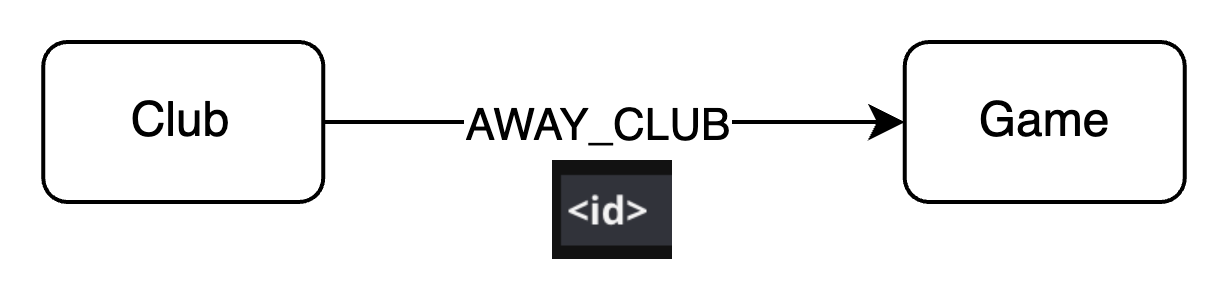
\includegraphics[width=\linewidth]{Project Template/Images/relationships/awayclub.png}
  \end{subfigure}
  \hfill
  \begin{subfigure}[b]{0.45\linewidth}
    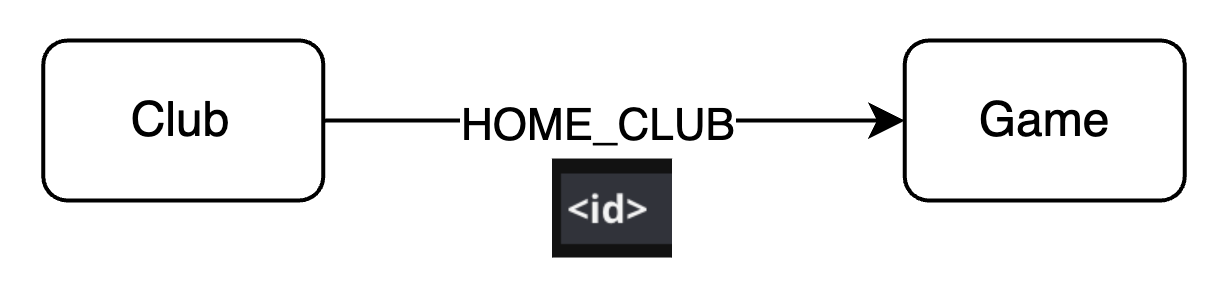
\includegraphics[width=\linewidth]{Project Template/Images/relationships/homeclub.png}
  \end{subfigure}

% Add some space before the next row
  \vspace{1em}

  \begin{subfigure}[b]{0.45\linewidth}
    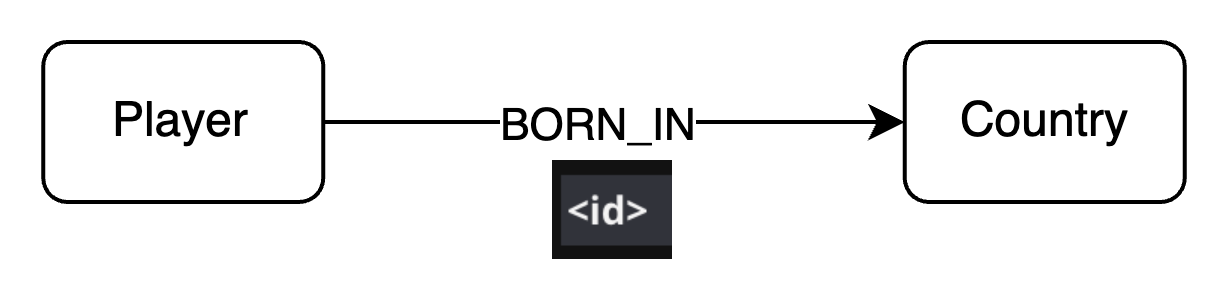
\includegraphics[width=\linewidth]{Project Template/Images/relationships/bornin.png}
  \end{subfigure}
  \hfill
  \begin{subfigure}[b]{0.45\linewidth}
    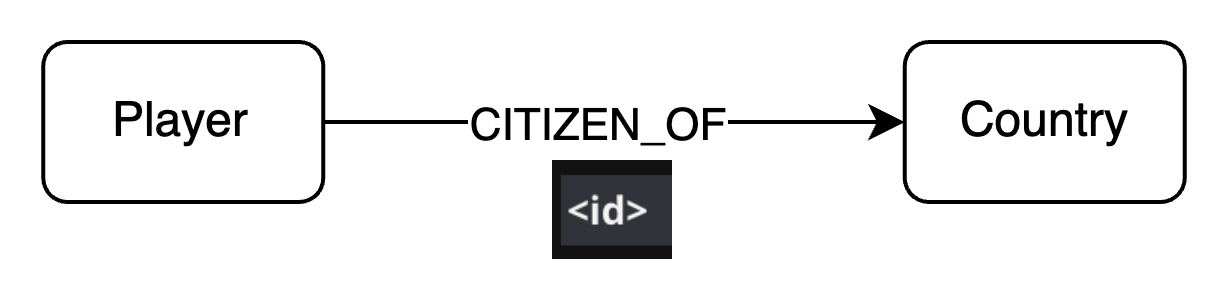
\includegraphics[width=\linewidth]{Project Template/Images/relationships/citizenof.png}
  \end{subfigure}
  
  % Add some space before the next row
  \vspace{1em}


    \begin{subfigure}[b]{0.45\linewidth}
    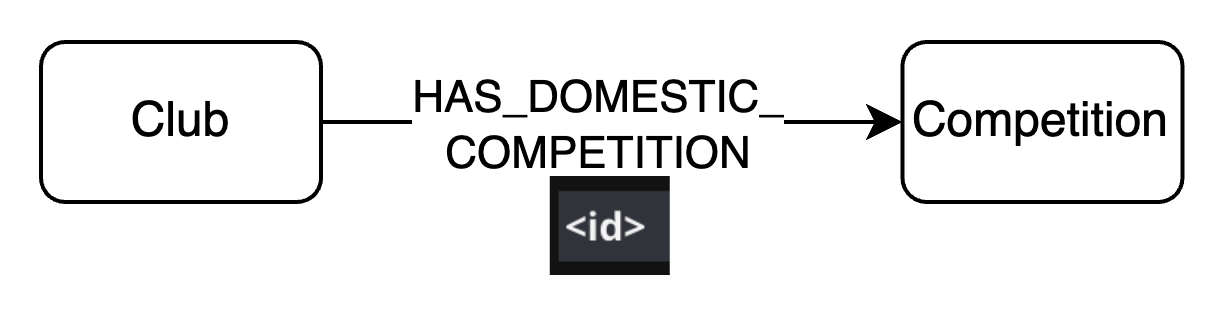
\includegraphics[width=\linewidth]{Project Template/Images/relationships/hasdomesticcompetition.png}
  \end{subfigure}
  \hfill
  \begin{subfigure}[b]{0.45\linewidth}
    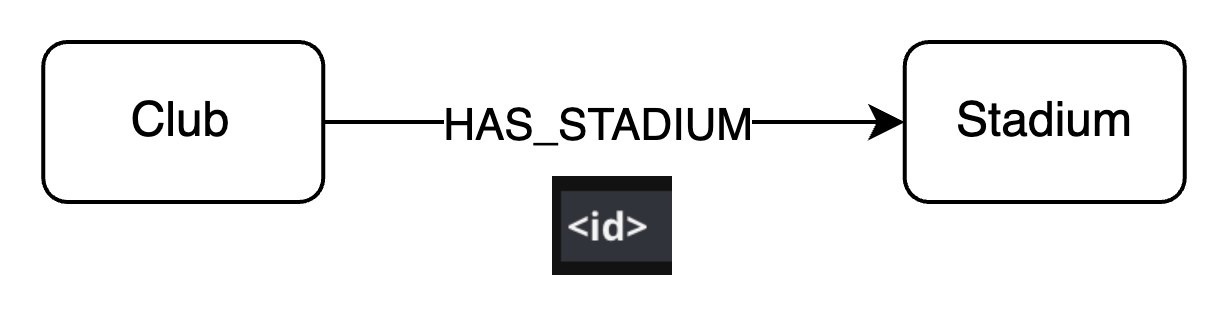
\includegraphics[width=\linewidth]{Project Template/Images/relationships/hasstadium.png}
  \end{subfigure}
  
  % Add some space before the next row
  \vspace{1em}



    \begin{subfigure}[b]{0.45\linewidth}
    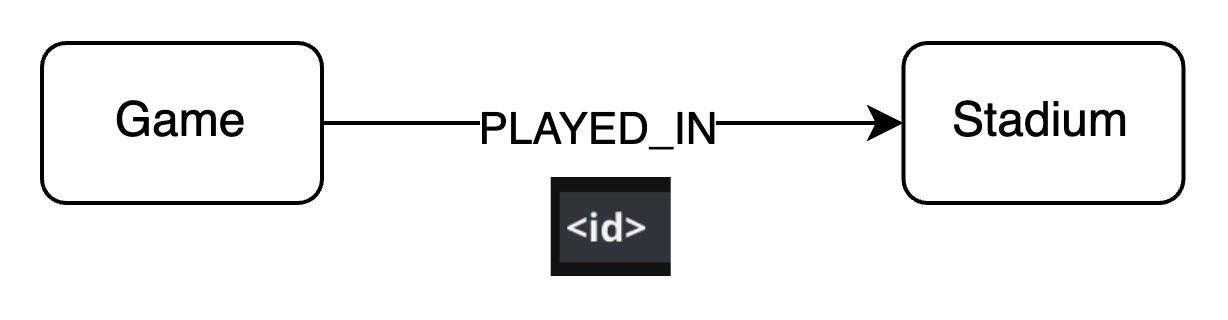
\includegraphics[width=\linewidth]{Project Template/Images/relationships/playedin.png}
  \end{subfigure}
  \hfill
  \begin{subfigure}[b]{0.45\linewidth}
    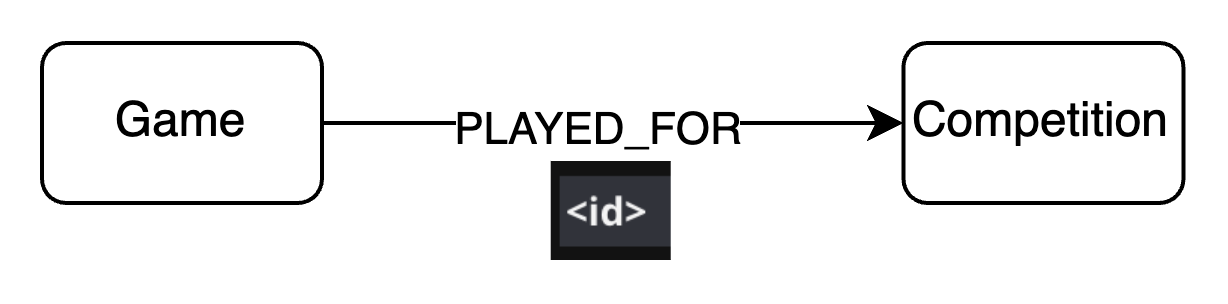
\includegraphics[width=\linewidth]{Project Template/Images/relationships/playsfor.png}
  \end{subfigure}
  
  % Add some space before the next row
  \vspace{1em}


    \begin{subfigure}[b]{0.45\linewidth}
    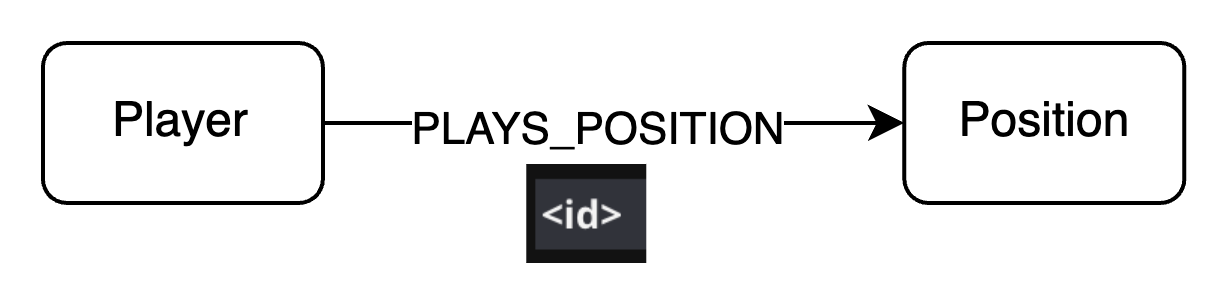
\includegraphics[width=\linewidth]{Project Template/Images/relationships/playsposition.png}
  \end{subfigure}
  \hfill
  \begin{subfigure}[b]{0.45\linewidth}
    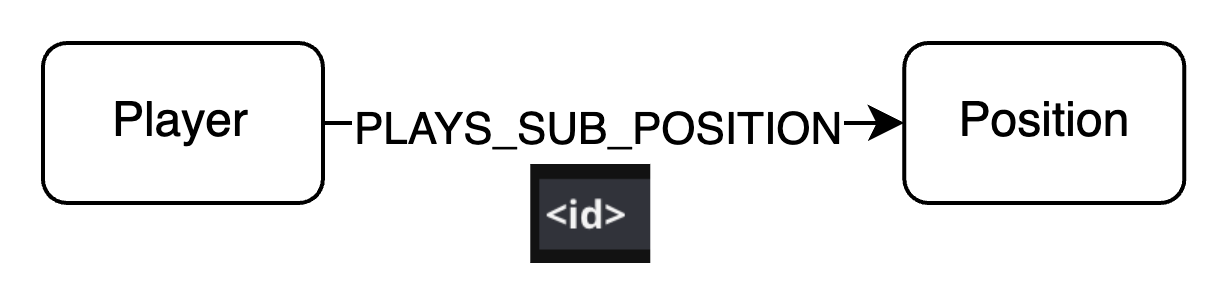
\includegraphics[width=\linewidth]{Project Template/Images/relationships/playssubposition.png}
  \end{subfigure}
  
  % Add some space before the next row
  \vspace{1em}


    \begin{subfigure}[b]{0.45\linewidth}
    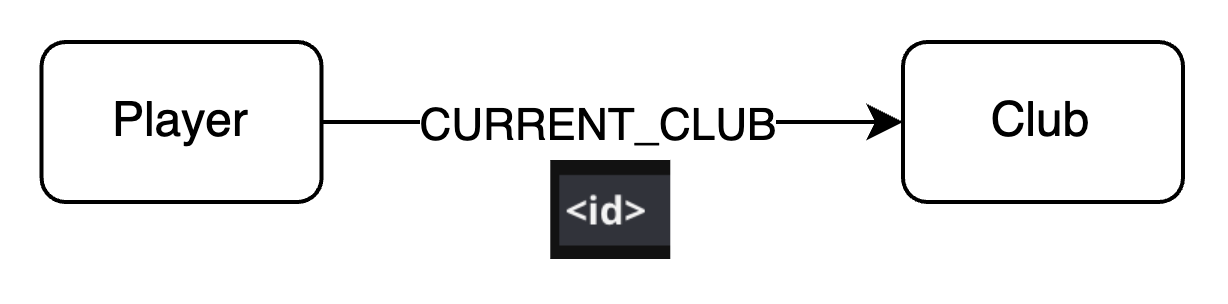
\includegraphics[width=\linewidth]{Project Template/Images/relationships/currentclub.png}
  \end{subfigure}
  \hfill
  \begin{subfigure}[b]{0.45\linewidth}
    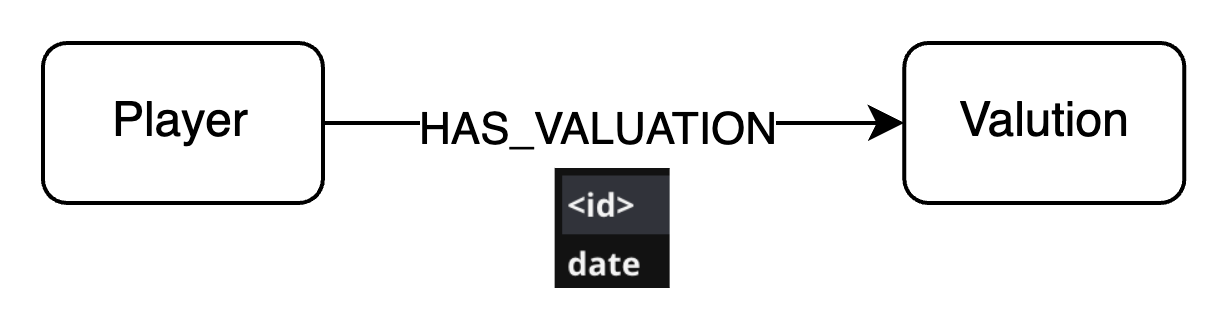
\includegraphics[width=\linewidth]{Project Template/Images/relationships/hasvaluation.png}
  \end{subfigure}
  
  % Add some space before the next row
  \vspace{1em}


    \begin{subfigure}[b]{0.45\linewidth}
    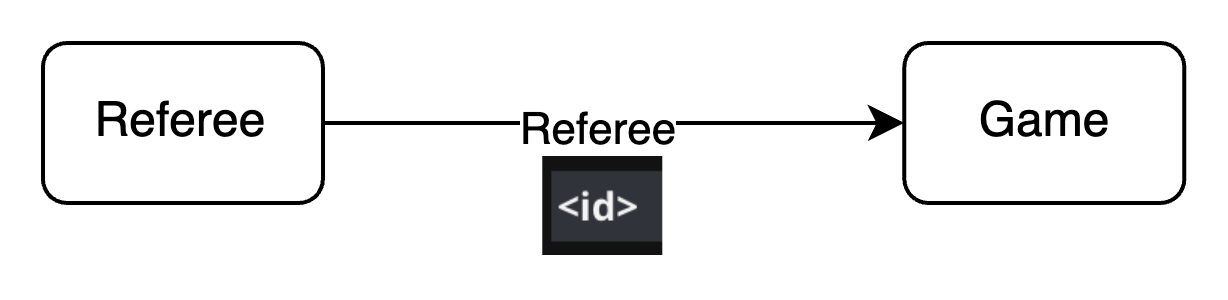
\includegraphics[width=\linewidth]{Project Template/Images/relationships/referee.png}
  \end{subfigure}
  \hfill
  \begin{subfigure}[b]{0.45\linewidth}
    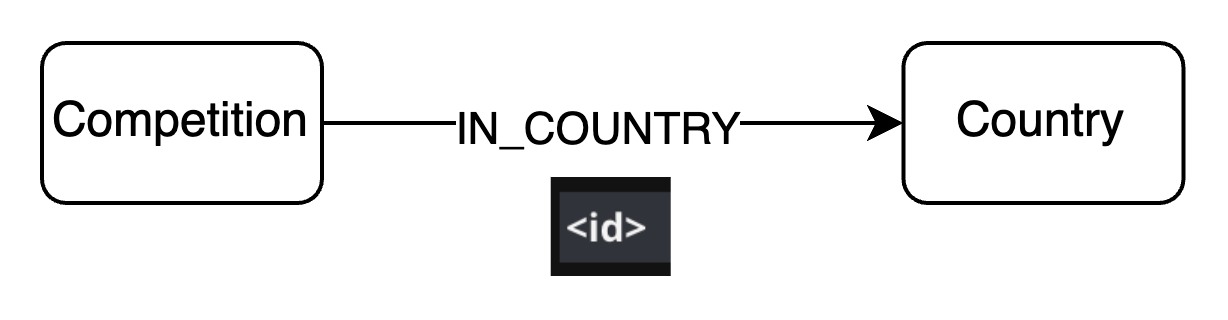
\includegraphics[width=\linewidth]{Project Template/Images/relationships/incountry.png}
  \end{subfigure}
  
  % Add some space before the next row
  \vspace{1em}

    \begin{subfigure}[b]{0.45\linewidth}
    \includegraphics[width=\linewidth]{Project Template/Images/relationships/appearances.png}
  \end{subfigure}
  
  
  \caption{Relationships and their attributes.}
\end{figure}

Except for the APPEARED\_IN relationship, all other relationships have only \textit{<id>} of type String, so their attribute will not be depicted with a table. Below, you can find the most important relationship APPEARED\_IN depicted with a table.

\subsection*{APPEARED\_IN (Relationship between Player and Game)}
\begin{longtable}{|p{4cm}|p{3cm}|p{8cm}|}
\hline
\textbf{Attribute} & \textbf{Type} & \textbf{Description} \\
\hline
\endhead
appearance\_id & Integer & Unique identifier for the appearance entry. \\
assists & Integer & Number of assists made by the player during the game. \\
date & Date & The date on which the appearance occurred. \\
goals & Integer & Number of goals scored by the player during the game. \\
minutes\_played & Integer & Total minutes played by the player in the game. \\
player\_club\_id & Integer & Unique identifier of the club the player appeared for. \\
red\_cards & Integer & Number of red cards received by the player during the game. \\
yellow\_cards & Integer & Number of yellow cards received by the player during the game. \\
\hline
\end{longtable}

As you can see the abundance of relationships, our dataset is very well-suited to be analysed by a graph network. The entities are interconnected to others with important relationships.




\chapter{Queries}

In this chapter, we will look at the queries we have written in detail, one by one. 

\section{Appearances in a Competition}

This query returns the players and their appearances grouped by competition and club. Competition Name is input.
If he has played in multiple clubs in the given competition, there will be multiple rows for the player.
Returns the Player\_ID, Player\_Name, Club\_Name, Appearances, Goals\_Scored, Assists, Yellow\_Cards, Red\_Cards, Minutes\_Played.

Return format:

\begin{lstlisting}[style=json]
{
    "Player_ID": 1,
    "Player_Name": "Lionel Messi",
    "Club_Name": "FC Barcelona",
    "Appereances": 10,
    "Goals_Scored": 5,
    "Assists": 3,
    "Yellow_Cards": 2,
    "Red_Cards": 0,
    "Minutes_Played": 900
}
\end{lstlisting}


Query:

\begin{lstlisting}[language=Cypher]
MATCH (p:Player)-[r:APPEARED_IN]->(g:Game)-[:HOME_CLUB|AWAY_CLUB]->(c:Club {club_id: r.player_club_id}),
(competition:Competition {name: "laliga"})
WHERE g.competition_id = competition.competition_id and c.name is not null
RETURN p.player_id AS Player_ID, p.name AS Player_Name, c.name AS Club_Name, COUNT(r) AS Appereances, SUM(r.goals) AS Goals_Scored, SUM(r.assists) AS Assists, SUM(r.yellow_cards) AS Yellow_Cards, SUM(r.red_cards) AS Red_Cards, SUM(r.minutes_played) AS Minutes_Played
ORDER BY Appereances DESC
\end{lstlisting}


Outcome:

\begin{figure}[H]
    \centering
    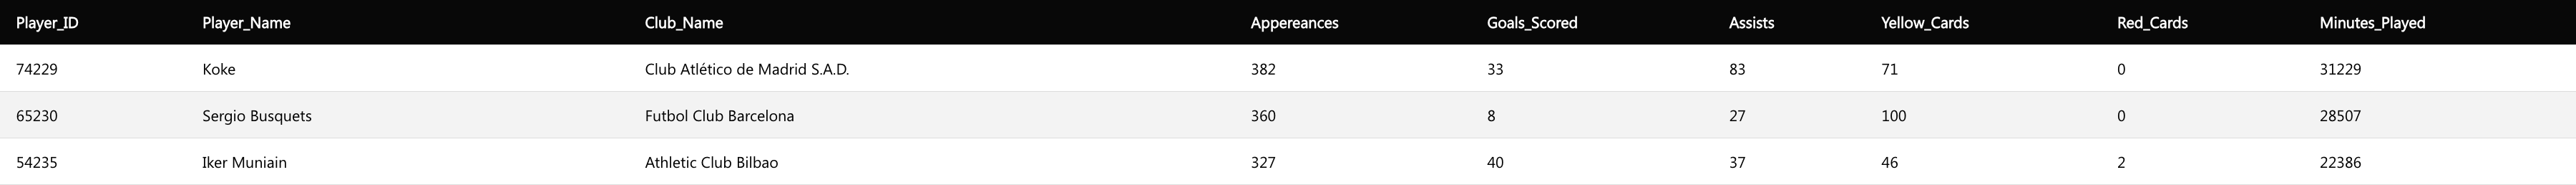
\includegraphics[width=\linewidth]{Project Template/Images/query_output/q1.png}
\end{figure}



\section{Goal and Assist Stats Against a Club}

This query returns the players and their goals and assists grouped by clubs.
If he has played against multiple clubs, there will be multiple rows for the player.
Returns the Player\_ID, Player\_Name, Own\_Club\_Name, Against\_Club\_Name, Goals\_Scored, Assists

Return format:
\begin{lstlisting}[style=json]
{
    "Player_ID": 1,
    "Player_Name": "Lionel Messi",
    "Own_Club_Name": "FC Barcelona",
    "Against_Club_Name": "Real Madrid",
    "Goals_Scored": 5,
    "Assists": 3
}
\end{lstlisting}


Query:

\begin{lstlisting}[language=Cypher]
MATCH (p:Player)-[r:APPEARED_IN]->(g:Game)-[:HOME_CLUB|AWAY_CLUB]->(c: Club {club_id: r.player_club_id}), 
(g)-[:HOME_CLUB|AWAY_CLUB]->(against_club: Club)
WHERE against_club.club_id <> c.club_id and c.name is not null and against_club.name is not null
WITH p.player_id AS Player_ID, p.name AS Player_Name, c.name AS Own_Club_Name, against_club.name AS Against_Club_Name,
SUM(r.goals) AS Goals_Scored, SUM(r.assists) AS Assists
WHERE Goals_Scored > 0
RETURN Player_ID, Player_Name, Own_Club_Name, Against_Club_Name, Goals_Scored, Assists
ORDER BY Goals_Scored DESC, Assists DESC
LIMIT(1000)
\end{lstlisting}


Outcome:

\begin{figure}[H]
    \centering
    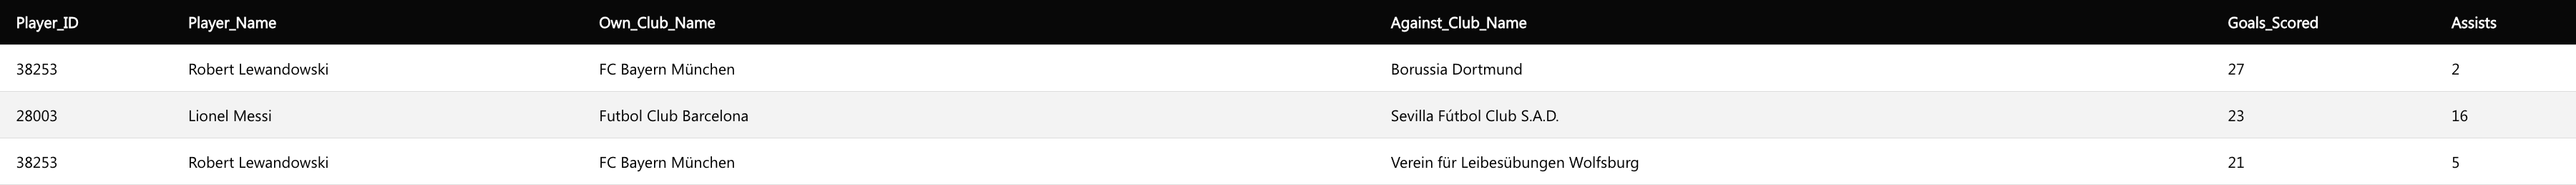
\includegraphics[width=\linewidth]{Project Template/Images/query_output/q2.png}
\end{figure}



\section{Two Players Against Each Other}
This query returns the players who played against each other the most.
Returns the Player\_1\_ID, Player\_1\_Name, player\_2\_id, Player\_2\_Name, Appereances\_Against

Return format:
\begin{lstlisting}[style=json]
{
    "Player_1_ID": 1,
    "Player_1_Name": "Lionel Messi",
    "player_2_id": 2,
    "Player_2_Name": "Cristiano Ronaldo",
    "Appereances_Against": 10
}
\end{lstlisting}


Query:

\begin{lstlisting}[language=Cypher]
MATCH (p1:Player)-[r1:APPEARED_IN]->(g:Game)<-[r2:APPEARED_IN]-(p2:Player), (competition:Competition {name: 'laliga'})
WHERE p1.player_id < p2.player_id and r1.player_club_id <> r2.player_club_id and g.competition_id = competition.competition_id
RETURN p1.player_id AS Player_1_ID, p1.name AS Player_1_Name, p2.player_id AS player_2_id, p2.name AS Player_2_Name, COUNT(r1) AS Appereances_Against
ORDER BY Appereances_Against DESC
LIMIT(1000)
\end{lstlisting}


Outcome:

\begin{figure}[H]
    \centering
    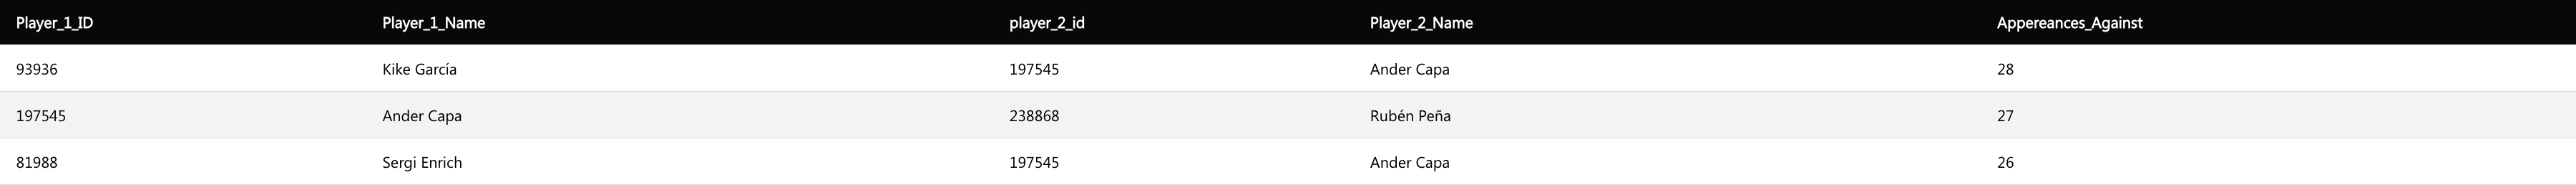
\includegraphics[width=\linewidth]{Project Template/Images/query_output/q3.png}
\end{figure}



\section{Average Age in a League}
This query returns the leagues and the number of players that have played in the league and the average age of the players in the games played, calculated from the date of the game minus the date of birth of the player. Returns the Competition\_ID, Competition\_Name, Total\_Number\_of\_Players, Average\_Age

Return format:
\begin{lstlisting}[style=json]
{
    "Competition_ID": 1,
    "Competition_Name": "La Liga",
    "Total_Number_of_Players": 100,
    "Average_Age": 25
}
\end{lstlisting}


Query:

\begin{lstlisting}[language=Cypher]
MATCH (p:Player)-[r:APPEARED_IN]->(g:Game)-[:PLAYED_FOR]->(c:Competition)
WHERE c.name IS NOT NULL
WITH c, p, g, r, duration.between(date(p.date_of_birth), date(g.date)).years AS age
RETURN c.competition_id AS Competition_ID, c.name AS Competition_Name, COUNT(DISTINCT p) AS Total_Number_of_Players, toInteger(avg(age)) AS Average_Age
ORDER BY Average_Age DESC
LIMIT(1000)
\end{lstlisting}


Outcome:
\begin{figure}[H]
    \centering
    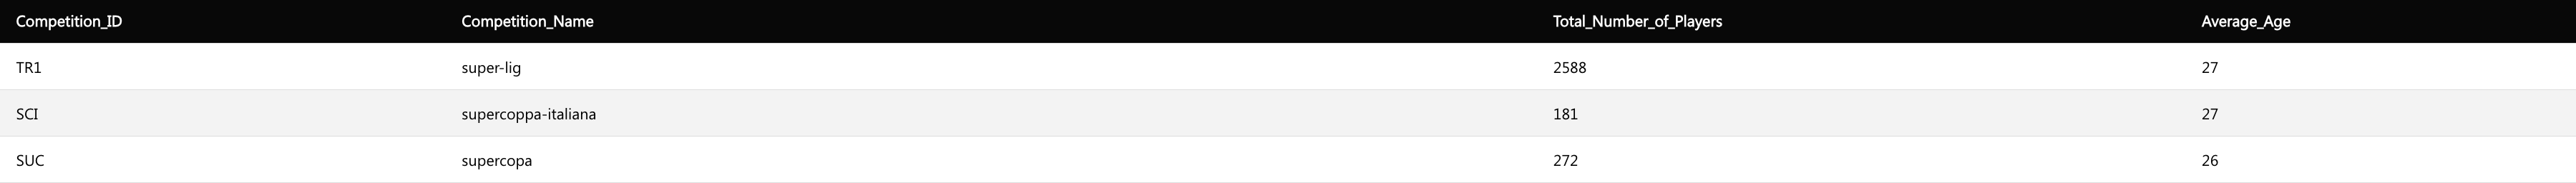
\includegraphics[width=\linewidth]{Project Template/Images/query_output/q4.png}
\end{figure}











\section{Player Wins Against a Club}
This query returns the players that got the most wins against a club. The competition name is given by input.
Returns the Player\_ID, Player\_Name, Own\_Club\_Name, Against\_Club\_name, Wins, Losses, Draws

Return format:
\begin{lstlisting}[style=json]
{
    "Player_ID": 1,
    "Player_Name": "Lionel Messi",
    "Own_Club_Name": "FC Barcelona",
    "Against_Club_name": "Real Madrid",
    "Wins": 10,
    "Losses": 5,
    "Draws": 3
}
\end{lstlisting}


Query:

\begin{lstlisting}[language=Cypher]
MATCH (p:Player)-[r:APPEARED_IN]->(g:Game)-[:HOME_CLUB|AWAY_CLUB]->(c:Club {club_id: r.player_club_id}),
(g)-[:HOME_CLUB|AWAY_CLUB]->(against_club: Club),
(competition:Competition {name: 'laliga'})
WHERE g.competition_id = competition.competition_id 
RETURN p.player_id AS Player_ID, p.name AS Player_Name, c.name AS Own_Club_Name, against_club.name AS Against_Club_name,
SUM(CASE WHEN g.home_club_goals > g.away_club_goals and c.club_id = g.home_club_id THEN 1
            WHEN g.away_club_goals > g.home_club_goals and c.club_id = g.away_club_id THEN 1
            ELSE 0 END) AS Wins,
SUM(CASE WHEN g.home_club_goals < g.away_club_goals and c.club_id = g.home_club_id THEN 1
            WHEN g.away_club_goals < g.home_club_goals and c.club_id = g.away_club_id THEN 1
            ELSE 0 END) AS Losses,
SUM(CASE WHEN g.home_club_goals = g.away_club_goals THEN 1 ELSE 0 END) AS Draws
ORDER BY Wins DESC, Losses ASC, Draws DESC
LIMIT(1000)
\end{lstlisting}


Outcome:
\begin{figure}[H]
    \centering
    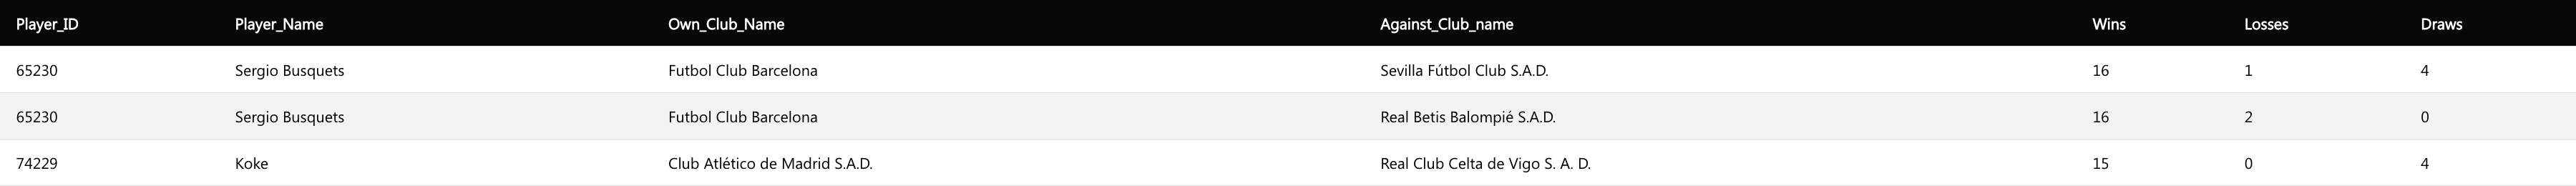
\includegraphics[width=\linewidth]{Project Template/Images/query_output/q5.png}
\end{figure}











\section{The Fixture with the Most Red Cards}
This query returns the pair clubs that played games with the highest red cards. Find red card from the appearances.
Returns the Club\_1\_Name, Club\_2\_Name, Red\_Cards

Return format:
\begin{lstlisting}[style=json]
{
    "Club_1_Name": "FC Barcelona",
    "Club_2_Name": "Real Madrid",
    "Matches_Played": 10,
    "Red_Cards": 10
}
\end{lstlisting}


Query:

\begin{lstlisting}[language=Cypher]
MATCH (c1:Club)<-[:HOME_CLUB|AWAY_CLUB]-(g:Game)-[:HOME_CLUB|AWAY_CLUB]->(c2:Club)
WHERE c1.club_id < c2.club_id and c1.name is not null and c2.name is not null
MATCH (p:Player)-[r:APPEARED_IN]->(g)
RETURN c1.name AS Club_1_Name, c2.name AS Club_2_Name, COUNT(DISTINCT g) AS Matches_Played, SUM(r.red_cards) AS Red_Cards
ORDER BY Red_Cards DESC, Matches_Played ASC
LIMIT(1000)
\end{lstlisting}


Outcome:
\begin{figure}[H]
    \centering
    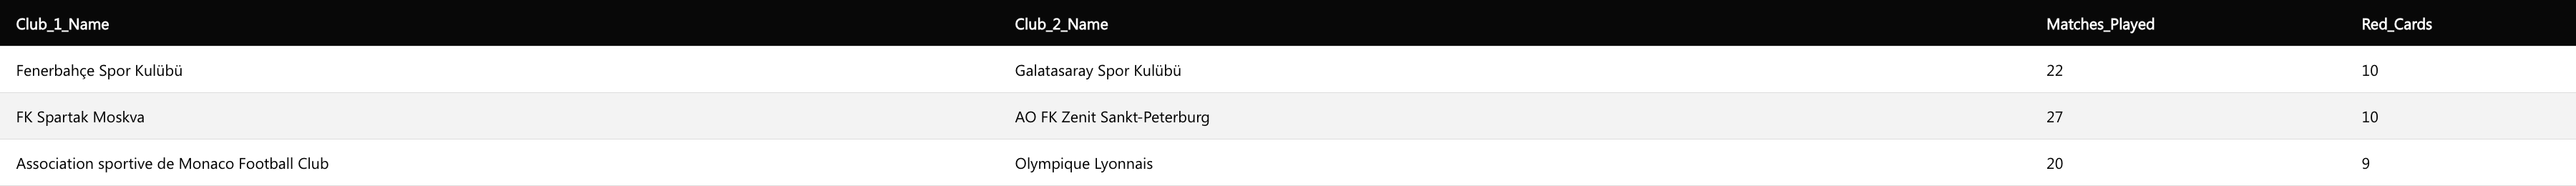
\includegraphics[width=\linewidth]{Project Template/Images/query_output/q6.png}
\end{figure}






\section{The Games with the Most Expensive Lineups}
This query returns the games with most average value of players. Calculates the average value of players in each game. The valuation of players is based on the market value of the player in the game. HAS\_VALUATION relationship with the closest and a past date is the real valuation of the player in the game.
Returns the Date, Home\_Club, Away\_Club, Average\_Valuation\_of\_Players.

Return format:
\begin{lstlisting}[style=json]
 {
    "Date": "FC Barcelona",
    "Home_Club": "Real Madrid",
    "Away_Club": 10,
    "Average_Valuation_of_Players": 10
}
\end{lstlisting}


Query:

\begin{lstlisting}[language=Cypher]
MATCH (g:Game)<-[:APPEARED_IN]-(p:Player),
(c_h:Club)<-[:HOME_CLUB]-(g), (c_a:Club)<-[:AWAY_CLUB]-(g)
WHERE c_h.name is not null and c_a.name is not null
WITH g, p, c_h, c_a
CALL {
    WITH g, p
    MATCH (p)-[r:HAS_VALUATION]->(v:Valuation)
    WHERE r.date <= g.date
    RETURN p.player_id AS player_id, g.game_id AS game_id, MAX(r.date) AS max_valuation_date
}
WITH g, p, max_valuation_date, c_h, c_a
MATCH (p)-[r:HAS_VALUATION {date: max_valuation_date}]->(v:Valuation)
RETURN g.date AS Date, c_h.name AS Home_Club, c_a.name AS Away_Club, ROUND(AVG(v.market_value_in_eur)) AS Average_Valuation_of_Players
ORDER BY Average_Valuation_of_Players DESC
LIMIT(1000)
\end{lstlisting}


Outcome:
\begin{figure}[H]
    \centering
    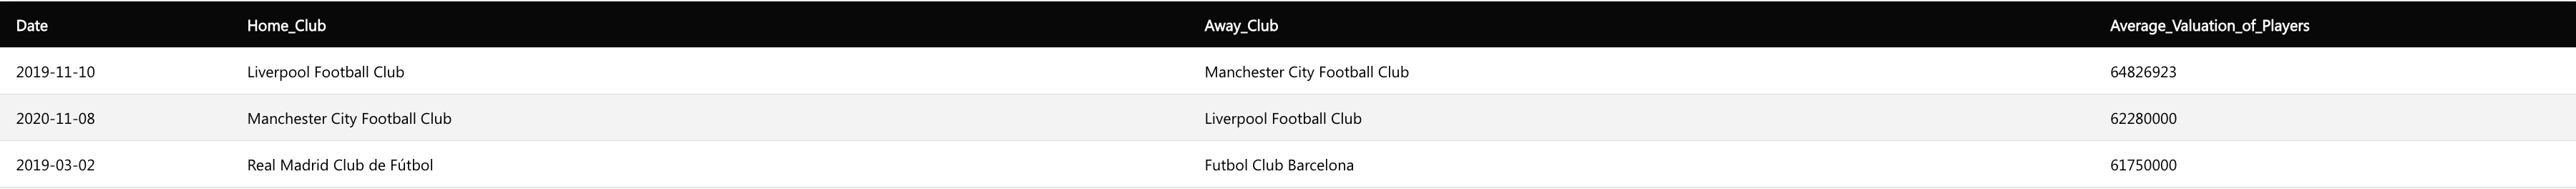
\includegraphics[width=\linewidth]{Project Template/Images/query_output/q7.png}
\end{figure}








\section{The Referee-Club Pairs with Most Bookings}
This query returns the referees with their most booked clubs. If the referee has booked multiple clubs, there will be multiple rows for the referee.
Returns the Referee\_Name, Club\_Name, Yellow\_Cards, Red\_Cards

Return format:
\begin{lstlisting}[style=json]
{
    "Referee_Name": "Mateu Lahoz",
    "Club_Name": "FC Barcelona",
    "Yellow_Cards": 10,
    "Red_Cards": 5
}
\end{lstlisting}


Query:

\begin{lstlisting}[language=Cypher]
MATCH (r:Referee)<-[:REFEREE]-(g:Game)<-[ap:APPEARED_IN]-(p:Player), (c:Club)
WHERE ap.player_club_id = c.club_id 
WITH r, c, SUM(ap.yellow_cards) AS totalYellow, SUM(ap.red_cards) AS totalRed
order by totalYellow+totalRed desc
WITH r, COLLECT({clubName: c.name, yellowCards: totalYellow, redCards: totalRed})[0] AS mostBookedClub
RETURN r.name AS Referee_Name, mostBookedClub.clubName AS Club_Name, mostBookedClub.yellowCards AS Yellow_Cards, mostBookedClub.redCards AS Red_Cards
order by Yellow_Cards + Red_Cards DESC, Red_Cards DESC, Yellow_Cards DESC
LIMIT(1000)
\end{lstlisting}


Outcome:
\begin{figure}[H]
    \centering
    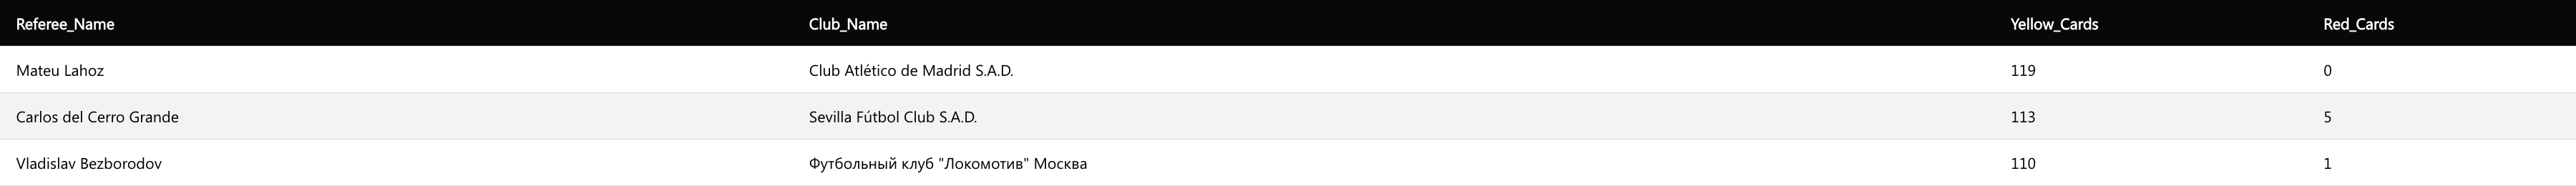
\includegraphics[width=\linewidth]{Project Template/Images/query_output/q8.png}
\end{figure}






\section{Goal and Assist Contribution per Minute}
This query returns the players with the lowest minutes played for a goal/assist, in a competition, per season of course.
Only players with more than 450 minutes played are considered. (roughly 5 matches)
Returns the Season, Competition\_ID, Player\_Name, Minutes\_Per\_Contibution, Total\_Minutes.

Return format:
\begin{lstlisting}[style=json]
{
    "Season": "2019",
    "Competition_ID": "CL",
    "Player_Name": "Rpbert Lewandowski",
    "Minutes_Per_Contibution": 42,
    "Total_Minutes": 450
}
\end{lstlisting}


Query:

\begin{lstlisting}[language=Cypher]
MATCH (g:Game)<-[ap:APPEARED_IN]-(p:Player), (comp:Competition)
WHERE g.competition_id = comp.competition_id
WITH g.season AS Season, comp.competition_id AS CompetitionID, p, SUM(ap.goals) AS TotalGoals, SUM(ap.assists) AS TotalAssists, SUM(ap.minutes_played) AS TotalMinutes
WHERE (TotalGoals + TotalAssists)>0 AND TotalMinutes>450
WITH Season, CompetitionID, p, TotalGoals, TotalAssists, TotalMinutes, (TotalMinutes * 1.0) / ((TotalGoals + TotalAssists) * 1.0) AS MinutesPerGA
ORDER BY MinutesPerGA ASC
RETURN Season, CompetitionID as Competition_ID, p.name AS Player_Name, ROUND(MinutesPerGA) as Minutes_Per_Contibution,TotalMinutes as Total_Minutes
LIMIT(1000)
\end{lstlisting}


Outcome:
\begin{figure}[H]
    \centering
    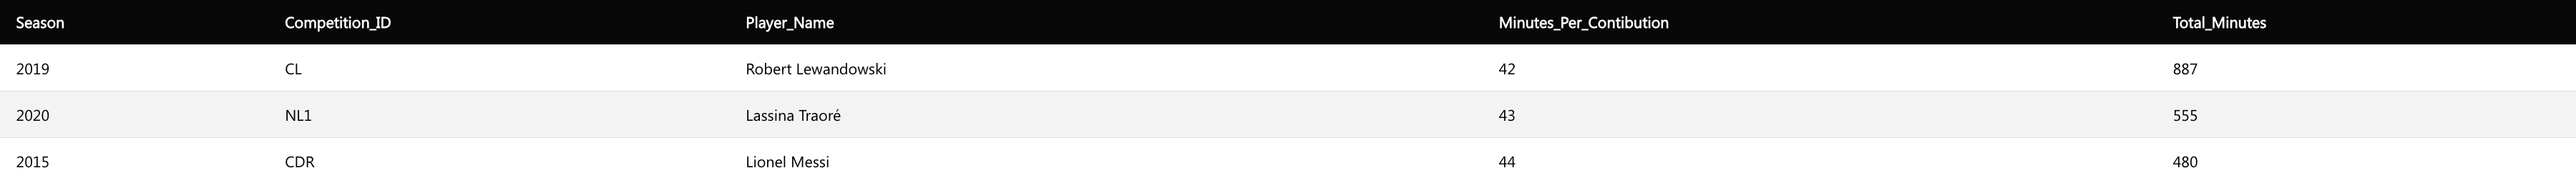
\includegraphics[width=\linewidth]{Project Template/Images/query_output/q9.png}
\end{figure}











\section{Players Carrying the Clubs}
This query returns the local heroes. Players that have the highest number of goals / team's goals in competition and season.
Returns the Player\_Name, Club\_Name, Competition\_Name, Season, Goals\_Scored\_By\_Player, Total\_Club\_Goals, Goals\_Scored, Ratio

Return format:
\begin{lstlisting}[style=json]
{
    "Player_Name": "Lionel Messi",
    "Club_Name": "FC Barcelona",
    "Competition_Name": "La Liga",
    "Season": "2019",
    "Goals_Scored_By_Player": 30,
    "Total_Club_Goals": 40,
    "Ratio": 0.75
}
\end{lstlisting}


Query:

\begin{lstlisting}[language=Cypher]
MATCH (comp:Competition), 
      (g:Game)-[:PLAYED_FOR]->(comp),
      (c:Club)<-[:HOME_CLUB|AWAY_CLUB]-(g)
where c.name is not null
WITH comp, c, g
// Calculate total goals for each club in the competition and season
WITH comp, c, g.season as season,
     SUM(CASE 
           WHEN g.home_club_id = c.club_id THEN g.home_club_goals 
           WHEN g.away_club_id = c.club_id THEN g.away_club_goals 
           ELSE 0 
         END) AS club_total_goals
// Match players and their goals in the same competition and season
WHERE club_total_goals>20
MATCH (p:Player)-[ap:APPEARED_IN]->(g:Game {season:season})-[:PLAYED_FOR]->(comp), 
      (g)-[:HOME_CLUB|AWAY_CLUB]->(c {club_id: ap.player_club_id})
RETURN p.name as Player_Name, 
       c.name as Club_Name, 
       comp.name as Competition_Name, 
       season as Season, 
       SUM(ap.goals) AS Goals_Scored_By_Player, 
       club_total_goals as Total_Club_Goals,
       ROUND(toFloat(SUM(ap.goals))/club_total_goals, 4) as Ratio
ORDER BY Ratio DESC
LIMIT(1000)
\end{lstlisting}


Outcome:
\begin{figure}[H]
    \centering
    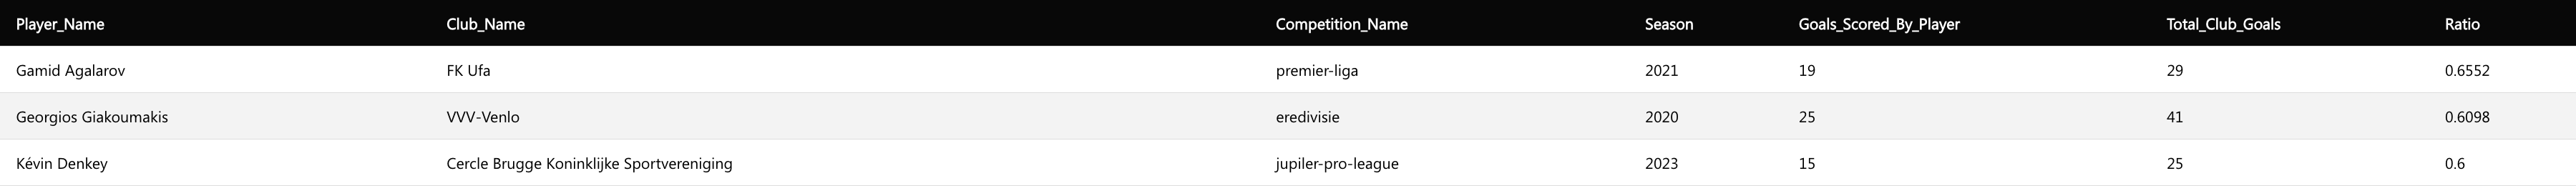
\includegraphics[width=\linewidth]{Project Template/Images/query_output/q10.png}
\end{figure}





\section{Given Country's Top Scorer}
This query returns the players with the most goal+assists for a given country and given age range.
Returns the Country\_Name, Player\_Name, Goals\_Scored, Assists, Minutes\_Played

Return format:
\begin{lstlisting}[style=json]
{
    "Country_Name": "Argentina",
    "Player_Name": "Lionel Messi",
    "Goals_Scored": 30,
    "Assists": 20,
    "Minutes_Played": 4500
}
\end{lstlisting}


Query:

\begin{lstlisting}[language=Cypher]
MATCH (p:Player)-[ap:APPEARED_IN]->(g:Game),
      (p)-[:CITIZEN_OF]->(c:Country)
WHERE c.country_name = 'Italy'
WITH p, ap, g, c,
duration.between(date(p.date_of_birth), date(g.date)).years AS age
WHERE age >= 15 AND age <= 40
RETURN c.country_name AS Country_Name, p.name AS Player_Name, SUM(ap.goals) AS Goals_Scored, SUM(ap.assists) AS Assists, SUM(ap.minutes_played) AS Minutes_Played
ORDER BY Goals_Scored DESC, Assists DESC, Minutes_Played ASC
LIMIT(1000)
\end{lstlisting}


Outcome:
\begin{figure}[H]
    \centering
    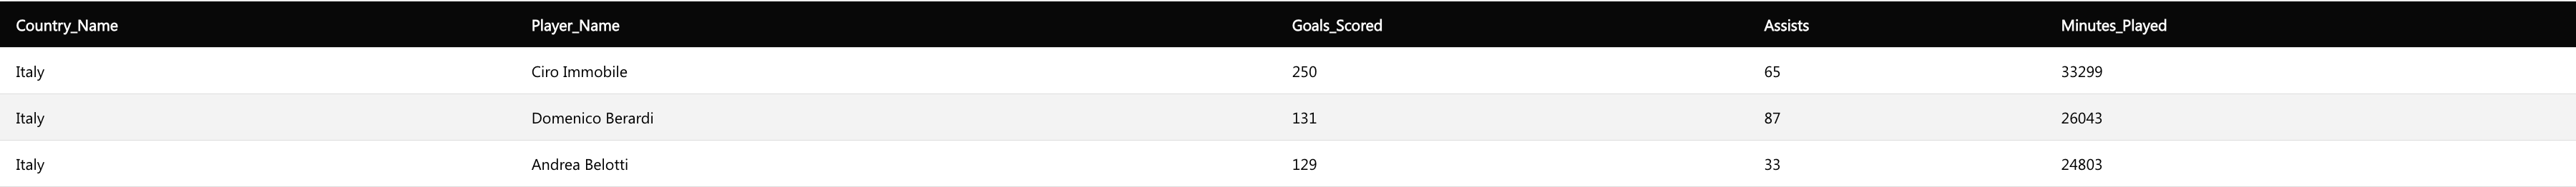
\includegraphics[width=\linewidth]{Project Template/Images/query_output/q11.png}
\end{figure}













\section{Manager Success with respect to Points Gained and Player Valuations}
Rate of valuations of players in games to points they get in the game, grouped by each manager. This query calculates the success of the manager. The higher the score, the better the manager. The score is calculated as follows:

\[
\text{Score} = \frac{\text{Average Point}}{\log(\text{Average Valuation})} \times 65
\]

The reason why we used \textit{log} is because Valuation is so much larger than Point, and we wanted to nerf its contribution to the score calculation. The reason to multiply by 65 is to scale it such that max score will be close to 10.

Group by manager name, sum of points from score, sum of valuation at that time.

Returns the Manager, Average\_Point, Matches\_Played, Average\_Valuation, Score

Return format:
\begin{lstlisting}[style=json]
{
    "Manager": "Lionel Messi",
    "Average_Point": 1.5,
    "Matches_Played": 100,
    "Average_Valuation": 1000000000,
    "Score": 0.5
}
\end{lstlisting}


Query:

\begin{lstlisting}[language=Cypher]
MATCH (g:Game)<-[a:APPEARED_IN]-(p:Player)
MATCH (c_h:Club)<-[:HOME_CLUB]-(g), (c_a:Club)<-[:AWAY_CLUB]-(g)
WHERE c_h.name IS NOT NULL AND c_a.name IS NOT NULL
WITH g, p, c_h, c_a,a

// Find the latest valuation for each player before the game
CALL {
    WITH g, p
    MATCH (p)-[r:HAS_VALUATION]->(v:Valuation)
    WHERE r.date <= g.date
    RETURN p.player_id AS player_id, g.game_id AS game_id, MAX(r.date) AS max_valuation_date
}

WITH g, p, max_valuation_date, c_h, c_a, a
MATCH (p)-[r:HAS_VALUATION {date: max_valuation_date}]->(v:Valuation)

// Aggregate and calculate average valuation for home and away teams
WITH g, 
     c_h.name AS home_club, 
     c_a.name AS away_club, 
     SUM(CASE WHEN a.player_club_id = c_h.club_id THEN v.market_value_in_eur ELSE 0 END) AS home_valuation,
     sum(CASE WHEN a.player_club_id = c_h.club_id THEN 1 ELSE 0 END) as home_player_count,
     SUM(CASE WHEN a.player_club_id = c_a.club_id THEN v.market_value_in_eur ELSE 0 END) AS away_valuation,
     sum(CASE WHEN a.player_club_id = c_a.club_id THEN 1 ELSE 0 END) as away_player_count
WITH g.date AS game_date, 
       home_club, 
       g.home_club_manager_name as home_manager,
       CASE WHEN g.home_club_goals>g.away_club_goals THEN 3 WHEN g.home_club_goals<g.away_club_goals THEN 0 ELSE 1 END as home_club_point,
       away_club, 
       g.away_club_manager_name as away_manager,
       CASE WHEN g.home_club_goals<g.away_club_goals THEN 3 WHEN g.home_club_goals>g.away_club_goals THEN 0 ELSE 1 END as away_club_point,
       home_valuation, 
       home_player_count,
       away_valuation,
       away_player_count
WITH home_manager, home_club_point, CASE WHEN home_player_count > 0 THEN toFloat(home_valuation)/home_player_count else NULL END as home_avg_valuation,
away_manager, away_club_point, CASE WHEN away_player_count > 0 THEN 
toFloat(away_valuation)/away_player_count else NULL END as away_avg_valuation
WITH [{manager: home_manager, point: home_club_point, avg_valuation: home_avg_valuation}, 
     {manager: away_manager, point: away_club_point, avg_valuation: away_avg_valuation}] AS managerList
UNWIND managerList AS managerData
WITH managerData.manager AS manager, managerData.point AS point, managerData.avg_valuation as average_valuation 
where average_valuation is not null
WITH  manager, avg(point) as avg_point, count(point) as Matches_Played, avg(average_valuation) as avg_valuation
WHERE Matches_Played > 30
return manager as Manager, Round(avg_point,1) as Average_Point, Matches_Played as Matches_Played, ROUND(avg_valuation) as Average_Valuation, ROUND(avg_point/log(avg_valuation)*65, 5) as Score
order by Score desc
limit(1000)
\end{lstlisting}


Outcome:
\begin{figure}[H]
    \centering
    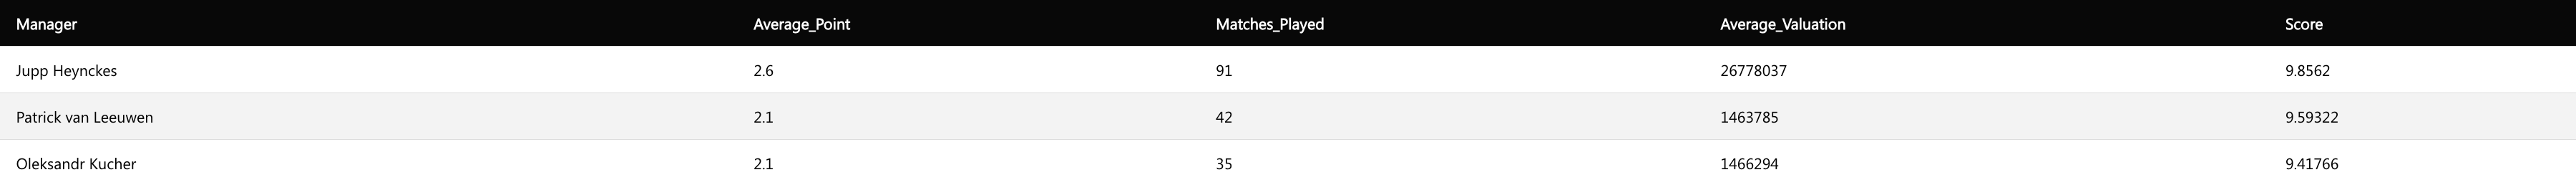
\includegraphics[width=\linewidth]{Project Template/Images/query_output/q12.png}
\end{figure}







\section{Average Goal per Game in Each Country}
This query returns the countries with most average goal per matches played year by year.
Calculated by (Competition)-[:IN\_COUNTRY]->(Country) relationship.
Input is year. Season attribute of Game node is used for year.
Game node has home club goals and away club goals attributes.

Returns the Country\_Name, Goals\_Scored, Matches\_Played, Average\_Goals

Return format:
\begin{lstlisting}[style=json]
{
    "Country_Name": "Argentina",
    "Goals_Scored": 10,
    "Matches_Played": 5,
    "Average_Goals": 2
}
\end{lstlisting}


Query:

\begin{lstlisting}[language=Cypher]
MATCH (g:Game)-[:PLAYED_FOR]->(c:Competition)-[:IN_COUNTRY]->(co:Country)
WHERE g.season = 2016
WITH co, g
WITH co, count(g) as Matches_Played, sum(g.home_club_goals + g.away_club_goals) as Goals_Scored
WHERE Matches_Played > 0
RETURN co.name as Country_Name, Goals_Scored as Goals_Scored, Matches_Played as Matches_Played, round(toFloat(Goals_Scored)/Matches_Played, 2) as Average_Goals
ORDER BY Average_Goals DESC, Goals_Scored DESC, Matches_Played ASC
\end{lstlisting}


Outcome:
\begin{figure}[H]
    \centering
    \includegraphics[width=\linewidth]{Project Template/Images/query_output/q13.png}
\end{figure}







\section{Stadium Aggressiveness with respect to Attendances and Red Cards}
This query returns the stadiums according to its heat. Heat is calculated by a Score measure that is:

\[
(Average\_Red\_Cards \times 10) + \log_{10}(Average\_Attendance)
\]

Retrieved by (p:Player)-[ai:APPEARED\_IN]->(g:Game)-[:PLAYED\_IN]->(s:Stadium) relationship.
ai.red\_cards attributes are used for red cards.
Input is year. Season attribute of Game node is used for year.
Game node has attendance attribute.

Returns the 
Stadium, 
Club,
Total\_Attendance,
Matches\_Played,
Average\_Attendance,
Red\_Cards,
Average\_Red\_Cards,
Score

Return format:
\begin{lstlisting}[style=json]
{
    "Stadium": "Camp Nou",
    "Club": "FC Barcelona",
    "Total_Attendance": 100000,
    "Matches_Played": 10,
    "Average_Attendance": 10000,
    "Red_Cards": 10,
    "Average_Red_Cards": 1,
    "Score": 10
}
\end{lstlisting}


Query:

\begin{lstlisting}[language=Cypher]
MATCH (g:Game)-[:PLAYED_IN]->(s:Stadium)<-[:HAS_STADIUM]-(c:Club)
where g.season = 2023
WITH s,c, g
MATCH (p:Player)-[ai:APPEARED_IN]->(g)
WITH s,c, g, sum(ai.red_cards) as Red_Cards
WITH s,c, count(g) as Matches_Played, sum(g.attendance) as total_attendance, sum(Red_Cards) as Red_Cards
WHERE Matches_Played > 5
WITH s.name as Stadium, c.name as Club, total_attendance as Total_Attendance, Matches_Played as Matches_Played, round(toFloat(total_attendance)/Matches_Played, 1) as Average_Attendance, Red_Cards as Red_Cards, round(toFloat(Red_Cards)/Matches_Played, 2) as Average_Red_Cards
WHERE Average_Attendance>0
RETURN Stadium, Club, Total_Attendance, Matches_Played, Average_Attendance, Red_Cards, Average_Red_Cards,
(Average_Red_Cards*10  + log10(Average_Attendance)) as Score
ORDER BY Score DESC
\end{lstlisting}


Outcome:
\begin{figure}[H]
    \centering
    \includegraphics[width=\linewidth]{Project Template/Images/query_output/q14.png}
\end{figure}




\section{Average Points Gained by Champions in Leagues}
This query returns the average point needed to be champion in a competition.
Returns the Competition, Average\_Championship\_Point


Return format:
\begin{lstlisting}[style=json]
{
    "Competition": "La Liga",
    "Average_Championship_Point": 80
}
\end{lstlisting}


Query:

\begin{lstlisting}[language=Cypher]
MATCH (comp:Competition)<-[:PLAYED_FOR]-(g:Game),
(c_h:Club)<-[:HOME_CLUB]-(g), (c_a:Club)<-[:AWAY_CLUB]-(g)
WHERE c_h.name IS NOT NULL AND c_a.name IS NOT NULL and EXISTS(()-[:HAS_DOMESTIC_COMPETITION]->(comp))
WITH g, comp.name as comp,
     c_h.name AS home_club, 
     c_a.name AS away_club
WITH g.date AS game_date, g.season as season, comp,
       home_club, 
       CASE WHEN g.home_club_goals>g.away_club_goals THEN 3 WHEN g.home_club_goals<g.away_club_goals THEN 0 ELSE 1 END as home_club_point,
       away_club, 
       CASE WHEN g.home_club_goals<g.away_club_goals THEN 3 WHEN g.home_club_goals>g.away_club_goals THEN 0 ELSE 1 END as away_club_point
WITH [{name: home_club, point: home_club_point, season: season, comp:comp}, 
     {name: away_club, point: away_club_point, season: season,comp:comp}] AS clubList
UNWIND clubList as club
with club.season as season, club.comp as competition, club.name as club_name, club.point as point
with season, competition, club_name, sum(point) as total_point
order by total_point desc
with distinct season, competition, collect(club_name) as clubs, collect(total_point) as points
WITH season, competition, clubs[0] as club, points[0] as point
RETURN competition as Competition, round(avg(point),2) as Average_Championship_Point
order by Average_Championship_Point desc
\end{lstlisting}


Outcome:
\begin{figure}[H]
    \centering
    \includegraphics[width=\linewidth]{Project Template/Images/query_output/q15.png}
\end{figure}











\section{Average Goal Difference for Each Manager}
This query returns the average goal difference for each coach.
Returns the Manager, Average\_Goal\_Difference, Matches\_Played


Return format:
\begin{lstlisting}[style=json]
{
    "Manager": "Lionel Messi",
    "Average_Goal_Difference": 1.5,
    "Matches_Played": 100
}
\end{lstlisting}


Query:

\begin{lstlisting}[language=Cypher]
MATCH (g:Game)<-[a:APPEARED_IN]-(p:Player)
MATCH (c_h:Club)<-[:HOME_CLUB]-(g), (c_a:Club)<-[:AWAY_CLUB]-(g)
WHERE c_h.name IS NOT NULL AND c_a.name IS NOT NULL and g.season = 2017
WITH g, p, c_h, c_a,a
// Find the latest valuation for each player before the game
CALL {
    WITH g, p
    MATCH (p)-[r:HAS_VALUATION]->(v:Valuation)
    WHERE r.date <= g.date
    RETURN p.player_id AS player_id, g.game_id AS game_id, MAX(r.date) AS max_valuation_date
}

WITH g, p, max_valuation_date, c_h, c_a, a
MATCH (p)-[r:HAS_VALUATION {date: max_valuation_date}]->(v:Valuation)

// Aggregate and calculate average valuation for home and away teams
WITH g, 
     c_h.name AS home_club, 
     c_a.name AS away_club
WITH g.date AS game_date, 
       home_club, 
       g.home_club_manager_name as home_manager,
       g.home_club_goals as home_club_goals,
       away_club, 
       g.away_club_manager_name as away_manager,
       g.away_club_goals as away_club_goals
WITH [{manager: home_manager, goals_scored: home_club_goals, goals_conceded: away_club_goals}, 
     {manager: away_manager, goals_scored: away_club_goals, goals_conceded: home_club_goals}] AS managerList
UNWIND managerList AS managerData
WITH managerData.manager AS manager, managerData.goals_scored AS goals_scored  , managerData.goals_conceded as goals_conceded
WITH goals_scored - goals_conceded as goal_difference, manager
WITH  manager, avg(goal_difference) as average_goal_difference, count(goal_difference) as Matches_Played
WHERE Matches_Played > 30
return manager as Manager, round(average_goal_difference, 2) as Average_Goal_Difference, Matches_Played as Matches_Played
order by Average_Goal_Difference desc, Matches_Played asc
\end{lstlisting}


Outcome:
\begin{figure}[H]
    \centering
    \includegraphics[width=\linewidth]{Project Template/Images/query_output/q16.png}
\end{figure}









\section{Average Valuation of Players per Country}
This query returns the average valuation of players in a given year for each country.
Returns the Country\_Name, Average\_Valuation, Number\_of\_Players


Return format:
\begin{lstlisting}[style=json]
{
    "Country_Name": "Argentina",
    "Average_Valuation": 1000000,
    "Number_of_Players": 100
}
\end{lstlisting}


Query:

\begin{lstlisting}[language=Cypher]
MATCH (p:Player)-[r:HAS_VALUATION]->(v:Valuation)
WITH p, v
WHERE duration.between(date(r.date), date({year:2005, month: 12, day:31})).months < 12
CALL {
    WITH p
    MATCH (p)-[r:HAS_VALUATION]->(v:Valuation)
    RETURN p.player_id AS player_id, MAX(r.date) AS max_valuation_date
}
WITH p, max_valuation_date
MATCH (p)-[r:HAS_VALUATION {date: max_valuation_date}]->(v_n:Valuation)
WITH distinct p, collect(v_n)[0] as v_n
MATCH (p)-[:CITIZEN_OF]->(c:Country)
WITH c, v_n
WITH c.country_name AS country_name, AVG(v_n.market_value_in_eur) AS average_valuation, count(v_n) as total_players
WHERE total_players > 5
return country_name as Country_Name, total_players as Number_of_Players, round(average_valuation) as Average_Valuation
ORDER BY Average_Valuation  DESC
\end{lstlisting}


Outcome:
\begin{figure}[H]
    \centering
    \includegraphics[width=\linewidth]{Project Template/Images/query_output/q17.png}
\end{figure}





\section{Goal Ratio of Players: Current Team / Total}
This query returns the players with the highest goal ratio for goals scored for the current club and scored in total.
Returns the Player\_ID, Player\_Name, Latest\_Club, Goals\_For\_Latest\_Club, Goals\_Scored, Goal\_Ratio


Return format:
\begin{lstlisting}[style=json]
{
    "Player_ID": 1,
    "Player_Name": "Lionel Messi",
    "Latest_Club": "FC Barcelona",
    "Goals_For_Latest_Club": 190,
    "Goals_Scored": 200,
    "Goal_Ratio": 0.95
}
\end{lstlisting}


Query:

\begin{lstlisting}[language=Cypher]
MATCH (p:Player)-[a:APPEARED_IN]->(g:Game)
WITH p, SUM(a.goals) AS Goals_Scored
MATCH (p)-[a_current:APPEARED_IN]->(:Game)
WHERE a_current.player_club_id = p.current_club_id
WITH p, Goals_Scored, SUM(a_current.goals) AS goals_for_current_club
WHERE Goals_Scored > 20 and goals_for_current_club > 0
RETURN p.player_id AS Player_ID, 
       p.name AS Player_Name,
       p.current_club_name AS Latest_Club,
       goals_for_current_club as Goals_For_Latest_Club,
       Goals_Scored as Goals_Scored,
       round(goals_for_current_club *1.0 / Goals_Scored, 2) AS Goal_Ratio
ORDER BY Goal_Ratio DESC, Goals_For_Latest_Club DESC
LIMIT(1000)
\end{lstlisting}


Outcome:
\begin{figure}[H]
    \centering
    \includegraphics[width=\linewidth]{Project Template/Images/query_output/q18.png}
\end{figure}






\section{Total Valuation of All Players Changes Over Time}
This query calculates the total valuation of all players in the entire dataset in a yearly basis.
Returns the year and total valuation in that year.

Using a simple Python script, we plotted a simple graph to see the valuation changes over time. 

\begin{figure}[H]
    \centering
    \includegraphics[width=0.5\linewidth]{valuationovertime.png}
\end{figure}

As you can see from the plot, the valuation of the players across the globe is increasing each and every year except for the COVID-19 era. Even with a simple query and a visualisation, we can see the effects of real world phenomena.


Return format:
\begin{lstlisting}[style=json]
{
    "Year": 2005,
    "Total_Valuation_Across_The_Globe": 10000000000
}
\end{lstlisting}


Query:

\begin{lstlisting}[language=Cypher]
WITH date("2004-01-01") AS startDate, // Start date
     date("2023-12-31") AS endDate // End date
WITH startDate, endDate,
     range(startDate.year, endDate.year) AS years
UNWIND years AS year
WITH date({year: year, month: 1, day: 1}) AS valuationYear

MATCH (p:Player)-[r:HAS_VALUATION]->(v:Valuation)
WITH p, v, valuationYear, r, 
     CASE 
         WHEN date(r.date).year <= valuationYear.year 
         THEN date(r.date).year 
         ELSE NULL 
     END AS valuationYearMatch
WHERE valuationYearMatch IS NOT NULL
WITH valuationYear, p, MAX(r.date) AS latestValuationDate
MATCH (p)-[r2:HAS_VALUATION {date: latestValuationDate}]->(v2:Valuation)
WITH valuationYear.year AS year, SUM(v2.market_value_in_eur) AS totalValuation
RETURN year as Year, totalValuation as Total_Valuation_Across_The_Globe
ORDER BY Year
\end{lstlisting}


Outcome:
\begin{figure}[H]
    \centering
    \includegraphics[width=\linewidth]{Project Template/Images/query_output/q19.png}
\end{figure}




\section{Games Played per Season for the Given Club}
This query calculates the total number of games played per season per club.
Returns the season, club name and number of games played.


Return format:
\begin{lstlisting}[style=json]
{
    "Season": 2005,
    "Matches_Played": 50,
    "Number_of_Distinct_Competitions": 3
}
\end{lstlisting}


Query:

\begin{lstlisting}[language=Cypher]
MATCH (c:Club {name: 'Liverpool Football Club'}) 
MATCH (g:Game)
WHERE g.home_club_id = c.club_id OR g.away_club_id = c.club_id
WITH g.season AS season, COUNT(g) AS numberOfGames, COLLECT(DISTINCT g.competition_id) AS competitions
RETURN season as Season, 
       numberOfGames as Matches_Played, 
       SIZE(competitions) AS Number_of_Distinct_Competitions
ORDER BY Season
\end{lstlisting}


Outcome:
\begin{figure}[H]
    \centering
    \includegraphics[width=\linewidth]{Project Template/Images/query_output/q20.png}
\end{figure}


\chapter{Extra Work}

For better demonstration purposes, we have deployed a \href{http://smbud.s3-website.eu-north-1.amazonaws.com/}{webpage} that includes the explanations and the outcomes of the queries. The tables stored in the pages are already sorted according to their queries. However, you can change the sorting simply by clicking the column name that you want to sort in any of the tables.

If you are not going to take a look at all 20 query demonstrations, we advise you to look at query #19 with the title \textit{'Prices go up and up! Unless...'}

You can find the related code from our repository: \href{https://github.com/mehmetemreakbulut/Football4J/tree/master}{Football4j}. 

Besides frontend code, you can find the code that sets up the Neo4j database environment using a pipeline.

Of course, the queries and the supplementary material (figures) used in this documentation can also be found in the repository.

% \chapter{Chapter one}
% \label{ch:chapter_one}%
% % The \label{...}% enables to remove the small indentation that is generated, always leave the % symbol.

% In this chapter additional useful information are reported.

% \section{Sections and subsections}
% \label{sec:section_name}
% Chapters are typically subdivided into sections and subsections, and, optionally,
% subsubsections, paragraphs and subparagraphs.
% All can have a title, but only sections and subsections are numbered.
% A new section is created by the command
% \begin{verbatim}
% \section{Title of the section}
% \end{verbatim}
% The numbering can be turned off by using \verb|\section*{}|.
% \\
% A new subsection is created by the command
% \begin{verbatim}
% \subsection{Title of the subsection}
% \end{verbatim}
% and, similarly, the numbering can be turned off by adding an asterisk as follows 
% \begin{verbatim}
% \subsection*{}
% \end{verbatim}

% \section{Equations}
% \label{sec:eqs}
% This section gives some examples of writing mathematical equations in your thesis.

% Maxwell's equations read:
% \begin{subequations}
%     \label{eq:maxwell}
%     \begin{align}[left=\empheqlbrace]
%     \nabla\cdot \bm{D} & = \rho, \label{eq:maxwell1} \\
%     \nabla \times \bm{E} +  \frac{\partial \bm{B}}{\partial t} & = \bm{0}, \label{eq:maxwell2} \\
%     \nabla\cdot \bm{B} & = 0, \label{eq:maxwell3} \\
%     \nabla \times \bm{H} - \frac{\partial \bm{D}}{\partial t} &= \bm{J}. \label{eq:maxwell4}
%     \end{align}
% \end{subequations}

% Equation~\eqref{eq:maxwell} is automatically labeled by \texttt{cleveref},
% as well as Equation~\eqref{eq:maxwell1} and Equation~\eqref{eq:maxwell3}.
% Thanks to the \verb|cleveref| package, there is no need to use \verb|\eqref|.
% Remember that Equations have to be numbered only if they are referenced in the text.

% Equations~\eqref{eq:maxwell_multilabels1}, \eqref{eq:maxwell_multilabels2}, \eqref{eq:maxwell_multilabels3}, and \eqref{eq:maxwell_multilabels4} show again Maxwell's equations without brace:
% \begin{align}
%     \nabla\cdot \bm{D} & = \rho, \label{eq:maxwell_multilabels1} \\
%     \nabla \times \bm{E} +  \frac{\partial \bm{B}}{\partial t} &= \bm{0}, \label{eq:maxwell_multilabels2} \\
%     \nabla\cdot \bm{B} & = 0, \label{eq:maxwell_multilabels3} \\
%     \nabla \times \bm{H} - \frac{\partial \bm{D}}{\partial t} &= \bm{J} \label{eq:maxwell_multilabels4}.
% \end{align}

% Equation~\eqref{eq:maxwell_singlelabel} is the same as before,
% but with just one label:
% \begin{equation}
%     \label{eq:maxwell_singlelabel}
%     \left\{
%     \begin{aligned}
%     \nabla\cdot \bm{D} & = \rho, \\
%     \nabla \times \bm{E} +  \frac{\partial \bm{B}}{\partial t} &= \bm{0},\\
%     \nabla\cdot \bm{B} & = 0, \\
%     \nabla \times \bm{H} - \frac{\partial \bm{D}}{\partial t} &= \bm{J}.
%     \end{aligned}
%     \right.
% \end{equation}

% \section{Figures, Tables and Algorithms}
% Figures, Tables and Algorithms have to contain a Caption that describe their content, and have to be properly reffered in the text.

% \subsection{Figures}
% \label{subsec:figures}

% For including pictures in your text you can use \texttt{TikZ} for high-quality hand-made figures,
% or just include them as usual with the command
% \begin{verbatim}
% \includegraphics[options]{filename.xxx}
% \end{verbatim}
% Here xxx is the correct format, e.g. \verb|.png|, \verb|.jpg|, \verb|.eps|, \dots.

% \begin{figure}[H]
%     \centering
%     \includegraphics[width=0.3\textwidth]{logo_polimi_scritta.eps}
%     \caption{Caption of the Figure to appear in the List of Figures.}
%     \label{fig:quadtree}
% \end{figure}

% Thanks to the \texttt{\textbackslash subfloat} command, a single figure, such as Figure~\ref{fig:quadtree},
% can contain multiple sub-figures with their own caption and label, e.g. \color{black} Figure~\ref{fig:polimi_logo1} and Figure~\ref{fig:polimi_logo2}. 

% \begin{figure}[H]
%     \centering
%     \subfloat[One PoliMi logo.\label{fig:polimi_logo1}]{
%         \includegraphics[scale=0.5]{Images/logo_polimi_scritta.eps}
%     }
%     \quad
%     \subfloat[Another one PoliMi logo.\label{fig:polimi_logo2}]{
%         \includegraphics[scale=0.5]{Images/logo_polimi_scritta2.eps}
%     }
%     \caption[Shorter caption]{This is a very long caption you don't want to appear in the List of Figures.}
%     \label{fig:quadtree2}
% \end{figure}


% \subsection{Tables}
% \label{subsec:tables}

% Within the environments \texttt{table} and  \texttt{tabular} you can create very fancy tables as the one shown in Table~\ref{table:example}.
% \begin{table}[H]
%     \caption*{\textbf{Title of Table (optional)}}
%     \centering 
%     \begin{tabular}{|p{3em} c c c |}
%     \hline
%     \rowcolor{bluepoli!40} % comment this line to remove the color
%      & \textbf{column 1} & \textbf{column 2} & \textbf{column 3} \T\B \\
%     \hline \hline
%     \textbf{row 1} & 1 & 2 & 3 \T\B \\
%     \textbf{row 2} & $\alpha$ & $\beta$ & $\gamma$ \T\B\\
%     \textbf{row 3} & alpha & beta & gamma \B\\
%     \hline
%     \end{tabular}
%     \\[10pt]
%     \caption{Caption of the Table to appear in the List of Tables.}
%     \label{table:example}
% \end{table}

% You can also consider to highlight selected columns or rows in order to make tables more readable.
% Moreover, with the use of \texttt{table*} and the option \texttt{bp} it is possible to align them at the bottom of the page. One example is presented in Table~\ref{table:exampleC}. 

% \begin{table}[H]
% \centering 
%     \begin{tabular}{|p{3em} | c | c | c | c | c | c|}
%     \hline
% %    \rowcolor{bluepoli!40}
%      & \textbf{column1} & \textbf{column2} & \textbf{column3} & \textbf{column4} & \textbf{column5} & \textbf{column6} \T\B \\
%     \hline \hline
%     \textbf{row1} & 1 & 2 & 3 & 4 & 5 & 6 \T\B\\
%     \textbf{row2} & a & b & c & d & e & f \T\B\\
%     \textbf{row3} & $\alpha$ & $\beta$ & $\gamma$ & $\delta$ & $\phi$ & $\omega$ \T\B\\
%     \textbf{row4} & alpha & beta & gamma & delta & phi & omega \B\\
%     \hline
%     \end{tabular}
%     \\[10pt]
%     \caption{Highlighting the columns}
%     \label{table:exampleC}
% \end{table}

% \begin{table}[H]
% \centering 
%     \begin{tabular}{|p{3em} c c c c c c|}
%     \hline
% %    \rowcolor{bluepoli!40}
%      & \textbf{column1} & \textbf{column2} & \textbf{column3} & \textbf{column4} & \textbf{column5} & \textbf{column6} \T\B \\
%     \hline \hline
%     \textbf{row1} & 1 & 2 & 3 & 4 & 5 & 6 \T\B\\
%     \hline
%     \textbf{row2} & a & b & c & d & e & f \T\B\\
%     \hline
%     \textbf{row3} & $\alpha$ & $\beta$ & $\gamma$ & $\delta$ & $\phi$ & $\omega$ \T\B\\
%     \hline
%     \textbf{row4} & alpha & beta & gamma & delta & phi & omega \B\\
%     \hline
%     \end{tabular}
%     \\[10pt]
%     \caption{Highlighting the rows}
%     \label{table:exampleR}
% \end{table}

% \subsection{Algorithms}
% \label{subsec:algorithms}

% Pseudo-algorithms can be written in \LaTeX{} with the \texttt{algorithm} and \texttt{algorithmic} packages.
% An example is shown in Algorithm~\ref{alg:var}.
% \begin{algorithm}[H]
%     \label{alg:example}
%     \caption{Name of the Algorithm}
%     \label{alg:var}
%     \label{protocol1}
%     \begin{algorithmic}[1]
%     \STATE Initial instructions
%     \FOR{$for-condition$}
%     \STATE{Some instructions}
%     \IF{$if-condition$}
%     \STATE{Some other instructions}
%     \ENDIF
%     \ENDFOR
%     \WHILE{$while-condition$}
%     \STATE{Some further instructions}
%     \ENDWHILE
%     \STATE Final instructions
%     \end{algorithmic}
% \end{algorithm} 

% \vspace{5mm}

% \section{Theorems, propositions and lists}

% \subsection{Theorems}
% Theorems have to be formatted as:
% \begin{theorem}
% \label{a_theorem}
% Write here your theorem. 
% \end{theorem}
% \textit{Proof.} If useful you can report here the proof.

% \subsection{Propositions}
% Propositions have to be formatted as:
% \begin{proposition}
% Write here your proposition.
% \end{proposition}

% \subsection{Lists}
% How to  insert itemized lists:
% \begin{itemize}
%     \item first item;
%     \item second item.
% \end{itemize}
% How to insert numbered lists:
% \begin{enumerate}
%     \item first item;
%     \item second item.
% \end{enumerate}

%-------------------------------------------------------------------------
%	APPENDICES
%-------------------------------------------------------------------------



% LIST OF FIGURES
\listoffigures


\cleardoublepage

\end{document}
